\documentclass[11pt]{article}
\usepackage[margin=0.88in]{geometry}
\usepackage{amsmath,amssymb,amsthm,booktabs,array,longtable}
\usepackage{mathtools,tikz}
\usetikzlibrary{arrows.meta}
\usepackage[T1]{fontenc}
\usepackage{xcolor}
\usepackage{hyperref}
\hypersetup{colorlinks=true,linkcolor=blue!45!black,citecolor=blue!45!black,urlcolor=blue!45!black}
\setlength{\parskip}{0.35em}
\setlength{\parindent}{0pt}
\setlength{\emergencystretch}{2em}
\newtheorem{proposition}{Proposition}
\newtheorem{theorem}{Theorem}
\newtheorem{corollary}[theorem]{Corollary}
\title{Agentic Progressive Verification for Hardware-Software Co-Design of AI Infrastructure}
\author{Research manuscript draft}
\date{October 8, 2026}
\begin{document}
\maketitle

\begin{abstract}
Design optimization across the software--hardware stack of AI infrastructure is a progressive process that begins with a workload computation graph and incrementally introduces software and hardware structures. Optimization solvers can search the resulting formulations, but feasibility alone does not establish that these structures preserve the computation. We propose \textbf{Agentic Progressive Verification}, a framework in which agents construct backward abstraction maps and candidate certificates connecting each refined formulation to its preceding, coarser representation. Formal obligations establish that every admitted refined design maps to a feasible coarse design and preserves its observable behavior and required completion. We prove sufficient local conditions for refinement, their composition across layers, and conditions for reusing earlier results after a formulation changes. A bounded prototype uses supplied certificate templates to check general matrix multiplication (GEMM) refinements involving partitioning, storage, asynchronous transfers, address mapping, partial tiles, limited resources, and operator composition. Its counterexamples expose errors that preserve earlier contracts, including stale buffer generations, omitted boundary work, and reachable resource deadlocks. Separate finite workload checks cover causal attention, prefill followed by decode, and one training transition, accepting 100 valid schedules and replaying faults in 16 injected-defect families. Across matched revision streams, exact-query reuse yields median paired full-check/reuse time ratios of $1.22$--$1.79\times$; caching completely checked finite workload groups yields $1.65$--$2.06\times$. A connected five-layer GEMM chain reduces cumulative verification from 92 to 27 solver calls and achieves a $2.51\times$ median paired speedup by inheriting accepted parent certificates. Savings remain workload- and change-dependent. The results show how newly introduced structures create verification obligations and when unchanged evidence can reduce repeated checking. Connecting workload and implementation layers through checked mappings and automating certificate construction remain open tasks.
\end{abstract}

\section{Introduction}
AI infrastructure requires coordinated optimization of software and hardware, from tensor operations and execution schedules to memory systems and microarchitecture. A natural approach is progressive refinement: begin with a workload computation graph and introduce implementation structure step by step. At each level, a constrained optimization formulation describes the available design choices. Mixed-integer programming (MIP), including mixed-integer linear programming (MILP), can express choices such as tile assignments, storage locations, resource configurations, and execution order.

The central challenge is ensuring that each refinement preserves the required computation. A solver establishes feasibility only with respect to the supplied constraints. If those constraints permit a live buffer to be overwritten or a consumer to run before a transfer completes, a feasible design can still compute the wrong result. Such errors arise from interactions introduced during refinement: a correct partition does not imply a correct storage schedule, and two correct operators can communicate through an incorrect shared-memory layout. Verification must establish the additional guarantees while retaining earlier results whose assumptions still hold.

Recent work provides complementary foundations. FLARE and SOVER combine large language models (LLMs) with formal reasoning to verify optimization reformulations~\cite{flare,sover}. TensorRight verifies tensor-graph rewrites, while BOLT verifies compiler-to-accelerator mappings through loop and layout correspondences~\cite{tensorright,bolt}. Refinement mappings and contract-based design establish how correctness composes as implementation details are introduced~\cite{refinementmaps,contracts}; incremental verification reuses results whose dependencies remain valid~\cite{incremental}. We build on these ideas to verify evolving families of feasible co-designs as software and hardware structures are added. Each refinement must preserve the workload's computation, even when it restricts design choices or changes cost estimates, while allowing unaffected guarantees to be reused.

\textbf{Our Contributions.} We propose \textbf{Agentic Progressive Verification}. Its central object is a backward abstraction map from a refined formulation to the preceding coarse formulation. Verification establishes that every feasible refined design has a feasible coarse interpretation and preserves the behavior and completion required at that level. These relationships compose from the final formulation back to the workload. Agents propose maps, invariants, and certificates; fixed formal obligations determine acceptance. Recorded premises determine whether an earlier result remains applicable after a change.

The prototype evaluates this organization using supplied templates and small, explicit computation and execution models. It combines satisfiability modulo theories (SMT) checks over fixed-shape design families with exhaustive exploration of finite executions. These experiments test structural preservation, progress, and reuse; automatic certificate construction by agents and checked mappings through all implementation layers remain research objectives.

Our contributions are summarized as follows:
\begin{itemize}
\item \textbf{A formal foundation for progressive formulation verification.} We define backward design maps and local obligations for feasibility, behavior, and completion, and prove their composition across refinement levels.
\item \textbf{A certificate-based agentic workflow.} We specify typed formulation interfaces and templates for maps, invariants, and progress arguments, with acceptance determined by explicit checks. A complete tensor-partition example connects the abstract method to executable verification conditions.
\item \textbf{Conditions and mechanisms for incremental reuse.} We establish when changed formulations can reuse earlier guarantees. The prototype measures reuse of accepted parent certificates along a connected refinement chain, as well as query and finite-execution reuse across revisions, while checking current prerequisites.
\end{itemize}

We evaluate correctness, verification efficiency, and workload coverage using eight structural benchmark groups and three workload components. GEMM refinements expose errors introduced by storage reuse, address mapping, partial tiles, and resource sharing, including three reachable deadlocks. Separate attention, inference, and training checks accept 100 valid schedules and produce replayed counterexamples for 16 faulty families. Across matched design revisions, reusing verification evidence reduces checking time by median paired factors of $1.22$--$1.79\times$ for structural benchmarks and $1.65$--$2.06\times$ for workload components, relative to full rechecking. A connected five-layer GEMM chain further achieves a $2.51\times$ median paired speedup, reducing cumulative solver calls from 92 to 27 by inheriting accepted parent certificates. These bounded experiments demonstrate useful reuse and coverage of distinct workload contracts; they do not yet establish large-model scalability or consistently faster checking in every run.

\section{Related Work}
Progressive verification for AI infrastructure connects several established research directions: optimization-model certification, semantic refinement, tensor-program verification, accelerator interfaces, and incremental proof reuse. The key comparison is what each method verifies and over which family of instances. Proving a rewrite rule, validating one implementation, and certifying every design admitted by a formulation provide different coverage.

\textbf{Optimization formulations and solver certificates.}
CvxLean formalizes correctness-preserving optimization reductions in Lean~\cite{cvxlean}. Conjure progressively translates abstract constraint specifications into concrete solver models~\cite{conjure}, making representation choice part of automated modeling. EquivaMap uses inferred correspondences to compare optimization formulations on instances~\cite{equivamap}. More recently, FLARE constructs machine-checkable MILP reformulation proofs, while SOVER combines LLM-assisted mappings with solver checks of feasibility and objective relationships~\cite{flare,sover}. These methods directly inform formulation verification. Complementary work checks solver results and internal transformations: VIPR provides independently checkable integer-programming certificates~\cite{vipr}, and Hoen et al. certify MIP-based presolve reductions for 0--1 integer programs using proof logging~\cite{presolve}. These guarantees address different boundaries. A certified solution satisfies the supplied model, and a certified reformulation preserves specified relationships to a reference model. Our additional obligation connects that model to workload behavior. Progressive design may intentionally restrict feasible choices, so preserving the original optimization problem in both directions is not always required.

\textbf{Refinement mappings and compositional design.}
Abadi and Lamport establish a foundational account of mappings from lower-level states to higher-level states, including the treatment of safety and liveness~\cite{refinementmaps}. Event-B similarly introduces implementation detail through refinement and explicit proof obligations~\cite{eventb}. Contract-based platform design is an especially close methodological precedent: Nuzzo et al. organize design as a sequence of refinements from requirements to implementations assembled from components, using contracts that separate environmental assumptions from component guarantees~\cite{contracts}. Thus, backward abstraction maps, progressive correctness, and compositional reasoning are established ideas. We specialize them to optimization formulations whose feasible assignments describe alternative software--hardware designs. Each refinement must both recover an admissible coarse design and preserve its observable computation. Shared storage, asynchronous completion, and bounded resources create compatibility and progress obligations that must accompany the mapping. Our compositional theorem states the conditions under which this specialization is sound.

\textbf{Verified compilation and tensor transformations.}
Translation validation checks the result of a compiler transformation against its input. Alive2 applies this approach to LLVM through bounded refinement checking~\cite{alive2}. For structured loops, Courant and Leroy mechanize polyhedral code generation, and Li, Liang, and Feng verify a validator for affine scheduling~\cite{polygen,polcert}. TensorRight verifies tensor-graph rewrite rules for arbitrary tensor ranks and sizes within its language: a proved rank bound reduces the general claim to finitely many symbolic verification obligations~\cite{tensorright}. This is stronger than simply testing small tensor instances. Tenspiler synthesizes tensor expressions and loop invariants, then uses an SMT prover to validate the lifted computation beyond the bounded synthesis domain~\cite{tenspiler}. These methods provide concrete mechanisms for our graph and tensor layers: reusable rewrite theorems, inferred invariants, and separately checked transformations. Our scope also includes the storage and execution structures admitted by later formulations. Conversely, our finite experiments do not establish TensorRight-style arbitrary-rank guarantees or replace verified compiler lowering.

\textbf{Accelerator interfaces and hardware--software verification.}
Instruction-Level Abstraction (ILA) specifies software-visible accelerator behavior and supports equivalence checking between abstract models and hardware implementations~\cite{ila}. Building on this interface, 3LA generates compiler and simulator support to enable application-level testing of accelerator designs~\cite{threela}. Such testing remains distinct from a universal correctness proof. BOLT is a particularly close recent verification approach: it aligns software and accelerator loops, relates their tensor layouts, and verifies a combined program against formal hardware semantics~\cite{bolt}. Its templates guide loop correspondence and layout invariants; the reported verifier instantiates configuration parameters with concrete values to handle nonlinear arithmetic. BOLT therefore addresses an important implementation bridge for our framework, while our formulation obligations quantify over the admitted design choices within their declared scope. Kami supplies modular hardware-verification foundations~\cite{kami}. COVERIF instead exploits firmware behavior through path-based symbolic execution and incremental solving to reduce hardware--software co-verification cost~\cite{coverif}. Together, these works show that abstraction, interface contracts, and implementation-level verification can be complementary. Any cost comparison must retain equivalent property coverage and include the remaining implementation checks.

\textbf{Optimization across computational and hardware levels.}
PLUTO uses integer linear optimization to select loop transformations~\cite{pluto}. CoSA encodes spatial-accelerator scheduling choices using MIP constraints derived from the computation and architecture~\cite{cosa}; Checkmate optimizes training rematerialization through MILP~\cite{checkmate}. These systems illustrate the modeling decisions that our method aims to verify. Mirage searches tensor programs across kernel, thread-block, and thread levels and uses a probabilistic equivalence procedure with theoretical guarantees~\cite{mirage}. Its evidence must be distinguished from a deterministic proof certificate. Exo 2 builds scheduling libraries from trusted primitives, and Exo-GPU verifies parallelism and synchronization against a sequential interpretation~\cite{exo2,exogpu}. Our method aims to maintain explicit preservation obligations as such optimization formulations acquire layouts, lifetimes, transfers, and hardware-resource choices. These systems also suggest reusable semantics and transformation libraries, rather than requiring every obligation to be constructed from scratch.

\textbf{Incremental verification and agent-assisted proof construction.}
Green normalizes constraints so their solutions can be reused within and across program analyses~\cite{green}. Leino and W\"ustholz use call-graph and control-flow dependencies to avoid rechecking unaffected program fragments~\cite{incremental}. Our query and finite-execution caches apply this established principle to successive co-design revisions. Their measured savings concern the recorded checks; they do not demonstrate general symbolic proof reuse across arbitrary workloads. For proof construction, LeanDojo provides programmatic interaction with Lean and retrieval of relevant premises for language-model-assisted proving~\cite{leandojo}. FLARE and SOVER bring related proposal-and-check workflows to optimization models~\cite{flare,sover}. We propose using agents to construct refinement maps, invariants, and repairs while retaining formal acceptance conditions. The present experiments use supplied templates and explicit backends, so autonomous proof discovery remains a system-development objective.

These foundations lead to our research question: can verification preserve the workload across an evolving family of feasible co-designs at a practical cost? Answering it requires explicit relationships between workload semantics, formulation constraints, and implementation structures, together with measurements of the cost of maintaining those relationships.

\section{Progressive Co-Design as Behavioral Refinement}\label{sec:formal}
The verification question is whether introducing software and hardware structure preserves the computation already specified at a coarser level. We first define the family of designs admitted by a formulation. We then state local proof obligations that are sufficient to preserve behavior, prove their soundness, and compose them across refinement levels. The proofs use established simulation reasoning; the proposed method constructs and reuses the corresponding certificates for co-design formulations.

\subsection{Workloads, formulations, and observable behavior}
A workload contract specifies admissible inputs and required observable behavior. Let $p\in\mathcal P$ denote workload parameters, such as tensor dimensions and batch size, and let $U(p)$ be the admissible runtime inputs. The set $W(p,u)$ contains the acceptable behaviors for input $u\in U(p)$. A behavior records externally visible events, final outputs, state updates, and completion status. Operators have fixed abstract semantics. Verification establishes preservation of the specified computation through tensor coverage, value flow, storage lifetime, execution ordering, and completion; floating-point accuracy, rounding error, and numerical stability are outside the scope of this work.

We consider terminating units of work: a kernel invocation, a bounded inference session, one decoding transition, or one training step. The contract excludes deadlock and nontermination for those units. A training input includes model parameters, optimizer state, gradients, and random-number state; its output includes the updated state. Appendix~\ref{app:training} gives the detailed training contract. An indefinitely running service requires a separate liveness argument beyond the terminating-unit theorem below.

The initial computation graph is checked against this workload contract. The reference semantics is specified independently of the optimization constraints: omitting a constraint must not erase the corresponding workload requirement. The following seven levels organize the introduction of structure; software and hardware choices can remain coupled throughout them.

\begin{center}
\small
\begin{tabular}{p{0.20\linewidth}p{0.29\linewidth}p{0.40\linewidth}}
\toprule
Refinement level & Representation and decisions & Principal proof obligations \\
\midrule
1: Workload specification & Required computation, admitted inputs and operator semantics & Independent reference contract; observable outputs and state changes \\
2: Computational graph & Operators, edges, parameter and state versions & Graph meaning and correspondence to the workload specification \\
3: Operator transformations & Fusion, decomposition, reduction partitioning & Preservation of abstract operator semantics and dependencies \\
4: Tensor execution mapping & Tiles, layouts, memory placement, processor mapping & Coverage, complete reductions, ownership, address maps, value lifetime \\
5: Instruction scheduling & Instruction selection, transfers, synchronization & Operand readiness, instruction semantics, visibility, progress \\
6: System architecture & Execution resources, memory hierarchy, interconnect & Resource compatibility, communication contracts, realizability \\
7: Microarchitecture & Pipelines, bank ports, queues, arbitration & Protocol behavior, capacity, backpressure, justified progress assumptions \\
\bottomrule
\end{tabular}
\end{center}

For the mathematics, the workload specification is the reference, and the remaining design representations have indices $\ell=0,\ldots,L$. The index 0 denotes the computation graph; the table gives $L=5$ for the complete sequence. Let $d_\ell$ contain the design variables at level $\ell$, and let $C_\ell(p,d_\ell)$ be its feasibility predicate. The formulation admits the design family
\begin{equation}
 F_\ell(p)=\{d_\ell\mid C_\ell(p,d_\ell)\}.
 \label{eq:family}
\end{equation}
A solver minimizes a predicted cost $J_\ell(p,d_\ell)$ over this family. The semantic proof concerns all admitted designs, independently of which one minimizes that cost. A finite menu can encode variable tile or hardware options in a MILP; products of unrestricted decision variables are not assumed linear.

Each formulation is stored as a typed model $\mathcal M_\ell$. It declares the design-variable domains, named constraint groups forming $C_\ell$, the objective $J_\ell$, and an operation description $P_\ell$. Substituting a design and an input into $P_\ell$ determines its operations, storage, and execution rules. The operational interpretation is
\begin{equation}
 \mathcal T_\ell(p,d_\ell,u)
 =\operatorname{Exec}_{\mathcal A_\ell}\bigl(P_\ell[p,d_\ell,u]\bigr),
 \label{eq:interpretation}
\end{equation}
where $\operatorname{Exec}$ is the fixed interpreter for the admitted operation constructors and $\mathcal A_\ell$ records the declared component and environment contracts. Integer indices, finite-width addresses, and tensor values have distinct types. A storage read returns the contents of the modeled location; it does not assume that the intended value is still there. Proving that correspondence is a refinement obligation. Section~\ref{sec:encoding} specifies how the model, interpreter, and solver encoding are connected.

For fixed parameters, design, and input, this transition system has states $S_\ell$, a nonempty set of initial states $I_\ell$, terminal states $T_\ell$ with no outgoing transitions, and a terminal observation function $O_\ell$. A transition $s\xrightarrow{w}_\ell s'$ emits a finite sequence $w$ of externally visible events. The empty sequence $\varepsilon$ denotes internal work. Terminal observations contain the final outputs and externally visible state.

A maximal execution either continues indefinitely or ends at a state without a successor. Ending at a nonterminal state is a failure. Let $B_\ell(p,d_\ell,u)$ be the behaviors of all maximal executions, including failure or divergence when present. Nonempty initialization and explicit failure behaviors prevent an unrealizable design from appearing correct through an empty behavior set. All transition systems are interpreted under declared environment assumptions; a refinement must justify the coarse assumptions using its concrete contracts.

A formulation is sound if every feasible design satisfies the workload for every admitted input:
\begin{equation}
 \forall p\in\mathcal P\;\forall d_\ell\in F_\ell(p)\;\forall u\in U(p),\qquad
 B_\ell(p,d_\ell,u)\subseteq W(p,u).
 \label{eq:sound}
\end{equation}
The quantifiers distinguish workload parameters, design choices, and runtime data. A fixed-shape proof restricts $\mathcal P$; testing sampled data does not establish the quantifier over $U(p)$.

\subsection{Backward abstraction and local proof obligations}
A backward abstraction map $\pi_\ell(p,\cdot)$ interprets a level-$\ell+1$ design as a level-$\ell$ design. It may recover graph operations from instruction sequences or logical tensors from tile and storage assignments. It must be defined for every feasible refined design and preserve feasibility:
\begin{equation}
 \forall p,d,\qquad C_{\ell+1}(p,d)
 \Longrightarrow C_\ell\bigl(p,\pi_\ell(p,d)\bigr).
 \label{eq:feas}
\end{equation}
The desired behavioral consequence is
\begin{equation}
 B_{\ell+1}(p,d,u)
 \subseteq B_\ell\bigl(p,\pi_\ell(p,d),u\bigr).
 \label{eq:behavior}
\end{equation}
We derive Equation~\ref{eq:behavior} from local conditions rather than assume it. The design map alone does not describe intermediate values or execution progress, so a certificate also supplies a relation between execution states.

Fix any admitted $p,u$ and feasible refined design $d$. In the following obligations, subscripts $f$ and $c$ denote its fine transition system and the coarse system selected by $\pi_\ell$. Let $R(s,a)$ relate a fine state $s\in S_f$ to a coarse state $a\in S_c$. Let $\rho(s,a)\in\mathbb N$ be a rank that measures progress during internal work. Write $a\xRightarrow[w]{m}_c a'$ for a path of exactly $m$ coarse transitions whose concatenated visible events are $w$. A zero-step path has $a'=a$ and $w=\varepsilon$.

The certificate establishes the following four execution obligations, in addition to Equation~\ref{eq:feas}. All state and event variables range over their respective typed domains.

\textbf{Initialization.} Each fine initial state has a coarse interpretation:
\begin{equation}
 \forall s_0\in I_f,\qquad \exists a_0\in I_c:\ R(s_0,a_0).
 \label{eq:init}
\end{equation}
\textbf{Step matching.} Every fine step has a finite coarse explanation with the same visible events. A step explained by no coarse progress must decrease the rank:
\begin{equation}
\begin{aligned}
 &\forall s,a,s',w,\quad R(s,a)\land s\xrightarrow{w}_f s'\\
 &\quad\Longrightarrow\exists a'\in S_c,\ m\in\mathbb N:\quad
 a\xRightarrow[w]{m}_c a'\ \land\ R(s',a')\\
 &\hspace{43mm}\land\bigl(m=0\Longrightarrow\rho(s',a)<\rho(s,a)\bigr).
\end{aligned}
 \label{eq:step}
\end{equation}

\textbf{Progress.} A represented fine state cannot stop before completing:
\begin{equation}
 \forall s,a,\quad R(s,a)\land s\notin T_f
 \Longrightarrow\exists s',w:\ s\xrightarrow{w}_f s'.
 \label{eq:progress}
\end{equation}
\textbf{Completion agreement.} Fine completion must correspond to coarse completion with the same final observation:
\begin{equation}
 \forall s,a,\quad R(s,a)\land s\in T_f
 \Longrightarrow a\in T_c\ \land\ O_f(s)=O_c(a).
 \label{eq:complete}
\end{equation}
The relation may include invariants about ownership, stored values, and completed work. These obligations quantify over all related states, a sufficient condition that avoids using an unproved reachability approximation. Initialization and step matching ensure that every reachable fine state encountered in the proof remains represented.

\subsection{Soundness of a local refinement}
The following theorem connects the local checks to the desired behavior guarantee. Step matching preserves observations, while the rank and progress conditions exclude infinite waiting and premature deadlock.
\begin{theorem}[Local refinement soundness]\label{thm:local}
Suppose Equations~\ref{eq:init}--\ref{eq:complete} hold for the fixed design and input, and every maximal execution of the coarse system terminates in $T_c$. Then every maximal fine execution terminates in $T_f$, and its visible history and terminal observation equal those of a maximal coarse execution. Consequently Equation~\ref{eq:behavior} holds.
\end{theorem}
\begin{proof}
Choose an arbitrary fine execution $s_0\xrightarrow{w_0}s_1\xrightarrow{w_1}\cdots$ with $s_0\in I_f$. Initialization and repeated step matching construct coarse states and path lengths satisfying
\begin{equation}
 R(s_i,a_i),\qquad
 a_i\xRightarrow[w_i]{m_i}_c a_{i+1},\qquad
 m_i=0\Longrightarrow\rho(s_{i+1},a_i)<\rho(s_i,a_i).
 \label{eq:matching-sequence}
\end{equation}
Let $\widehat r$ be the concatenation of these coarse paths, and let $\operatorname{tr}(r)$ denote the visible event sequence of an execution $r$. For every finite prefix of $n$ fine steps,
\begin{equation}
 |\widehat r_n|=K_n:=\sum_{i=0}^{n-1}m_i,
 \qquad
 \operatorname{tr}(\widehat r_n)=w_0\cdots w_{n-1}
 =\operatorname{tr}(r_n).
 \label{eq:trace-prefix}
\end{equation}
If the fine execution is finite and maximal, its last state $s_n$ has no successor. Equations~\ref{eq:progress} and~\ref{eq:complete} imply
\begin{equation}
 \neg\exists s',w:\ s_n\xrightarrow{w}_f s'
 \Longrightarrow s_n\in T_f
 \Longrightarrow a_n\in T_c\ \land\ O_f(s_n)=O_c(a_n).
 \label{eq:finite-completion}
\end{equation}
Thus $\widehat r_n$ is a maximal coarse execution with the same complete behavior.

Suppose instead that the fine execution is infinite. Since each $m_i$ is a nonnegative integer, there are two cases. If $(K_n)$ is unbounded, the matched paths concatenate into an infinite coarse execution, contrary to the coarse termination premise. If $(K_n)$ is bounded, it eventually stops increasing:
\begin{equation}
 \sup_n K_n<\infty
 \Longrightarrow\exists N\;\forall i\ge N:\ m_i=0\ \land\ a_i=a_N.
\end{equation}
The rank must then decrease at every remaining fine step. For all $k\in\mathbb N$,
\begin{equation}
 \rho(s_N,a_N)\ge\rho(s_{N+k},a_N)+k\ge k.
\end{equation}
Taking $k=\rho(s_N,a_N)+1$ yields a contradiction. Both infinite cases are impossible. Every maximal fine execution therefore terminates, and the finite-case argument establishes behavior inclusion.
\end{proof}

The backward direction refers to the design abstraction map. The execution proof follows fine steps and constructs matching coarse paths; this is a simulation argument. The rank permits finite silent cleanup after coarse completion, but excludes endless internal waiting. Hardware arbitration or transfer progress used by the proof must follow from the specified execution contract; an unstated fairness assumption cannot supply Equation~\ref{eq:progress} or the rank argument. The termination premise ranges over all maximal paths of the stated transition system; preservation of an externally imposed fairness restriction requires a separate argument.

\subsection{Composition across the software--hardware stack}
For fixed $p$, compose the backward maps as
\begin{equation}
 \Pi_{0:L}=\pi_0\circ\pi_1\circ\cdots\circ\pi_{L-1},
 \label{eq:map-composition}
\end{equation}
where the parameter argument is suppressed and the rightmost map acts first. The composite map interprets a final design as a computation-graph design.

\begin{theorem}[Progressive formulation soundness]\label{thm:composition}
Suppose the computation-graph formulation satisfies Equation~\ref{eq:sound}, with terminating workload behaviors. Suppose every refinement satisfies Equation~\ref{eq:feas} and the obligations of Theorem~\ref{thm:local}, for every admitted parameter, feasible fine design, and admissible input, under compatible environment assumptions. Then
\begin{equation}
 \forall p\in\mathcal P,\ d\in F_L(p),\ u\in U(p),\qquad
 B_L(p,d,u)\subseteq B_0\bigl(p,\Pi_{0:L}(d),u\bigr)\subseteq W(p,u).
 \label{eq:composed-soundness}
\end{equation}
\end{theorem}
\begin{proof}
Fix arbitrary $p$, $d_L\in F_L(p)$, and $u\in U(p)$. Define the coarser designs backward:
\begin{equation}
 d_\ell:=\pi_\ell(p,d_{\ell+1}),\qquad \ell=L-1,\ldots,0.
\end{equation}
Repeated feasibility preservation gives
\begin{equation}
 C_L(p,d_L)\Longrightarrow C_{L-1}(p,d_{L-1})
 \Longrightarrow\cdots\Longrightarrow C_0(p,d_0).
\end{equation}
Soundness of the computation-graph formulation establishes termination and $B_0(p,d_0,u)\subseteq W(p,u)$. Induction from $\ell=0$ to $L-1$, applying Theorem~\ref{thm:local}, establishes termination at each next level and
\begin{equation}
 B_{\ell+1}(p,d_{\ell+1},u)\subseteq B_\ell(p,d_\ell,u).
\end{equation}
Consequently,
\begin{equation}
 B_L(p,d_L,u)\subseteq B_{L-1}(p,d_{L-1},u)
 \subseteq\cdots\subseteq B_0(p,d_0,u)\subseteq W(p,u).
\end{equation}
Because $d_0=\Pi_{0:L}(d_L)$ and the chosen parameters, design, and input were arbitrary, Equation~\ref{eq:composed-soundness} follows.
\end{proof}

Soundness is distinct from nonemptiness. For each parameter instance supported by certified optimization, a feasible witness or constructive existence proof must additionally establish
\begin{equation}
 \forall p\in\mathcal P_{\mathrm{supported}},\qquad
 \exists d_L:\ C_L(p,d_L).
 \label{eq:witness}
\end{equation}
A failed solver search does not prove infeasibility. Likewise, a refinement can correctly restrict the design space without preserving its original optimum. A reverse map or an appropriate coverage and objective argument is required if optimization equivalence is claimed.

\section{Agentic Construction and Checking of Refinement Proofs}\label{sec:method}
\subsection{System organization and evidence flow}
Figure~\ref{fig:system} places progressive verification within the overall agentic design-automation loop. A shared candidate population retains formulations, linked designs, assumptions, and evidence. The optimization branch searches those formulations; the verification branch constructs and checks their refinement certificates. Both return information to the refinement agent. Formal acceptance and measured performance remain separate results attached to the same candidate.

\begin{figure}[htbp]
\centering
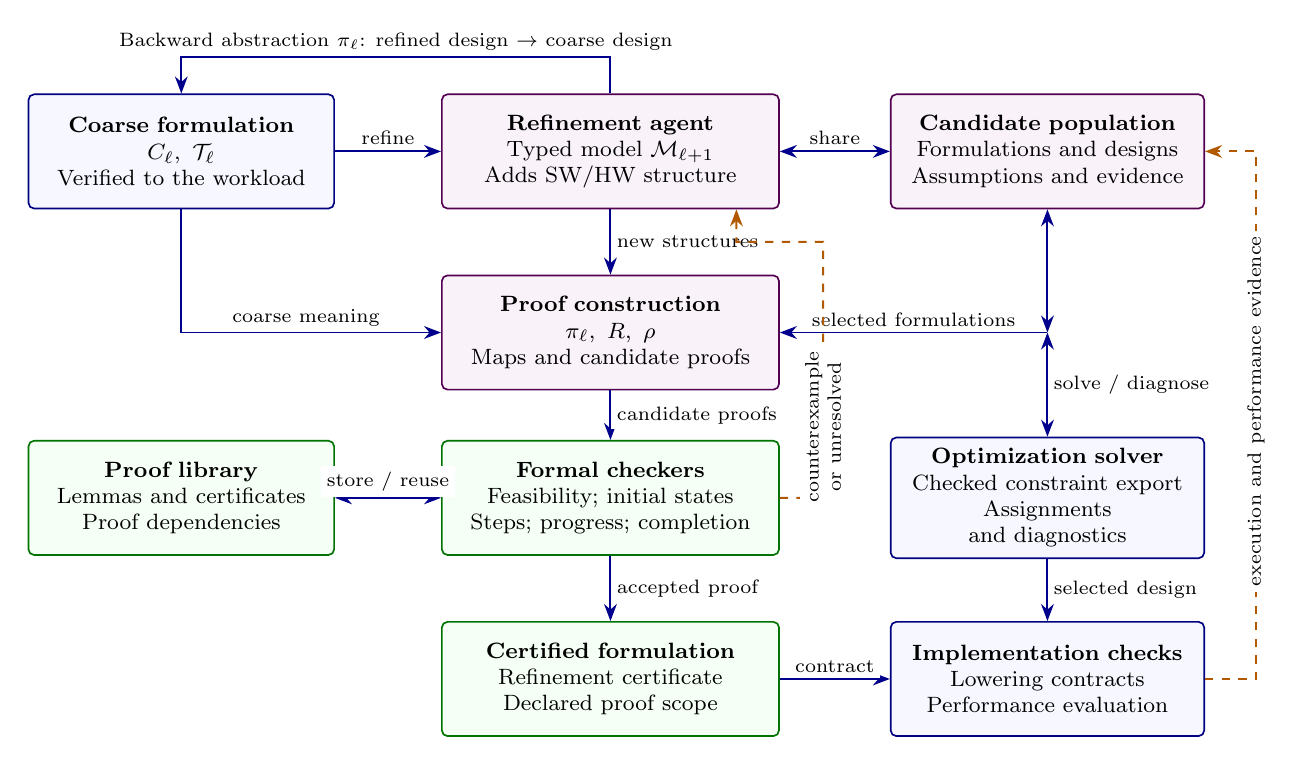
\begin{tikzpicture}[
 x=1cm,y=1cm,>=Stealth,
 box/.style={draw=blue!50!black,fill=blue!3,rounded corners=2pt,
             line width=0.6pt,align=center,font=\footnotesize,minimum height=1.45cm,
             inner sep=4pt,text width=3.6cm},
 agent/.style={box,draw=violet!65!black,fill=violet!5,text width=4.0cm},
 checked/.style={box,draw=green!45!black,fill=green!4},
 flow/.style={->,line width=0.7pt,draw=blue!55!black},
 feedback/.style={->,dashed,line width=0.7pt,draw=orange!70!black},
 lab/.style={font=\scriptsize,align=center,fill=white,inner sep=2pt}
]
\node[box] (coarse) at (2.0,7.4) {\textbf{Coarse formulation}\\$C_\ell,\ \mathcal T_\ell$\\Verified to the workload};
\node[agent] (agent) at (7.45,7.4) {\textbf{Refinement agent}\\Typed model $\mathcal M_{\ell+1}$\\Adds SW/HW structure};
\node[agent,text width=3.7cm] (population) at (13.0,7.4) {\textbf{Candidate population}\\Formulations and designs\\Assumptions and evidence};
\draw[flow] (coarse.east) -- node[lab,above]{refine} (agent.west);
\draw[flow,<->] (agent.east) -- node[lab,above]{share} (population.west);
\draw[flow] (agent.north) -- (7.45,8.6) -- node[lab,above]{Backward abstraction $\pi_\ell$: refined design $\rightarrow$ coarse design} (2.0,8.6) -- (coarse.north);

\node[agent] (proof) at (7.45,5.1) {\textbf{Proof construction}\\$\pi_\ell,\ R,\ \rho$\\Maps and candidate proofs};
\draw[flow] (agent.south) -- node[lab,right]{new structures} (proof.north);
\draw[flow] (coarse.south) |- node[lab,pos=.74,above]{coarse meaning} (proof.west);
\draw[flow,<->] (population.south) -- (13.0,5.1);
\draw[flow] (13.0,5.1) -- node[lab,above]{selected formulations} (proof.east);

\node[checked] (cache) at (2.0,3.0) {\textbf{Proof library}\\Lemmas and certificates\\Proof dependencies};
\node[checked,text width=4.0cm] (check) at (7.45,3.0) {\textbf{Formal checkers}\\Feasibility; initial states\\Steps; progress; completion};
\node[box,text width=3.7cm] (solve) at (13.0,3.0) {\textbf{Optimization solver}\\Checked constraint export\\Assignments and diagnostics};
\draw[flow] (proof.south) -- node[lab,right]{candidate proofs} (check.north);
\draw[flow,<->] (cache.east) -- node[lab,above]{store / reuse} (check.west);
\draw[flow,<->] (13.0,5.1) -- node[lab,right]{solve / diagnose} (solve.north);
\draw[feedback] (check.east) -- (10.15,3.0) -- (10.15,6.25) -- (9.05,6.25) -- ([xshift=1.6cm]agent.south);
\node[lab,rotate=90] at (10.15,3.9) {counterexample\\or unresolved};

\node[checked,text width=4.0cm] (certified) at (7.45,0.7) {\textbf{Certified formulation}\\Refinement certificate\\Declared proof scope};
\node[box,text width=3.7cm] (evaluate) at (13.0,0.7) {\textbf{Implementation checks}\\Lowering contracts\\Performance evaluation};
\draw[flow] (check.south) -- node[lab,right]{accepted proof} (certified.north);
\draw[flow] (solve.south) -- node[lab,right]{selected design} (evaluate.north);
\draw[flow] (certified.east) -- node[lab,above]{contract} (evaluate.west);
\draw[feedback] (evaluate.east) -- (15.65,0.7) -- (15.65,7.4) -- (population.east);
\node[lab,rotate=90] at (15.65,4.1) {execution and performance evidence};
\end{tikzpicture}
\caption{Progressive verification within agentic hardware--software co-design. The upper arrow shows the backward abstraction direction. Agents propose maps and proofs; formal checkers establish the refinement obligations. Both branches consume the same typed model, with a checked translation to solver constraints. Solid arrows carry models, proofs, selected designs, and solver diagnostics; dashed arrows return evidence for revision. Implementation and performance checks remain explicit after formulation certification.}\label{fig:system}
\end{figure}

The agent receives the accepted coarse model, the proposed fine model, and a record of the introduced structures. Each new tile, buffer, instruction, or resource retains its relationship to the operation or logical value it implements. These relationships guide map construction but are not trusted as proofs. An exploratory candidate may be solved or simulated before its proof is complete; only checked obligations support a correctness-certified result.

\subsection{Identify the refinement level and specify its semantics}\label{sec:encoding}
The seven levels in Section~\ref{sec:formal} describe \emph{what becomes concrete}: workload specification, computational graph, operator transformations, tensor execution mapping, instruction scheduling, system architecture, and microarchitecture. The procedure in this section describes \emph{how each refinement is verified}. It repeats at every level and can also check several successive refinements within one level, such as first tiling a tensor and then allocating reusable buffers. Table~\ref{tab:refinement-maps} identifies the coarse meaning to recover and the additional evidence required at each boundary.

\begin{table}[htbp]
\centering\small
\begin{tabular}{p{0.23\linewidth}p{0.32\linewidth}p{0.36\linewidth}}
\toprule
Refinement boundary & Backward interpretation & Newly required evidence \\
\midrule
Workload $\rightarrow$ graph & Interpret graph outputs and state updates as the specified workload transition & Operator composition, required outputs, and state versions match the independent specification \\
Graph $\rightarrow$ transformed operators & Interpret fused or decomposed operations as the original graph region & Rewrites preserve operator meaning and producer--consumer dependencies \\
Operators $\rightarrow$ tensor mapping & Recover logical tensor elements and reductions from tiles, layouts, and placements & Complete coverage, exact-once contributions, correct addresses, and valid buffer lifetimes \\
Tensor mapping $\rightarrow$ instruction schedule & Interpret instruction sequences and transfer events as logical tensor operations & Operands are ready, synchronization preserves visibility, and execution completes \\
Schedule $\rightarrow$ system architecture & Interpret distributed resource and communication actions as the scheduled operations & Resource assignments and communication protocols satisfy the schedule's assumptions \\
Architecture $\rightarrow$ microarchitecture & Interpret pipeline, bank, and queue transitions as architectural operations & Instruction effects, conflict handling, and arbitration preserve behavior and progress \\
\bottomrule
\end{tabular}
\caption{Applying the same verification procedure across the refinement levels. The backward interpretation guides construction of the design map and execution-state relation; it is not itself a proof. Each row requires the local obligations of Section~\ref{sec:formal}.}\label{tab:refinement-maps}
\end{table}

Hardware choices can remain symbolic at earlier levels and become concrete later. These boundaries therefore organize proof obligations without requiring software decisions to be finalized before hardware exploration. If a later resource choice changes an earlier layout or schedule, the agent revises the affected formulations and rechecks their dependent guarantees. A candidate's record identifies both its refinement level and the exact preceding model to which its certificate applies.

At the selected boundary, the first step is to state exactly what the refinement introduces and what remains fixed. The input is an accepted coarse model, a proposed fine model, and their declared parameter and input domains. For example, replacing logical tensors with reusable buffers introduces addresses, reads, and writes while retaining the meaning of the tensor operations. The proposed model interface gives the verifier and optimizer one source of variable definitions and constraints. Its operation constructors cover pure tensor operations, index transformations, storage allocation and access, issue and completion events, and finite resource protocols. Each constructor has a fixed transition rule, observation rule, and list of required contracts. For example, a load uses the current contents at its decoded address, while an asynchronous transfer has distinct issue and completion events. Absence of interference or eventual completion is not assumed merely because an agent labels a transfer correct. A new operation constructor requires a checked semantic definition before it can support certification.

Let $\mathcal D_\ell(p)$ be the declared domain of design assignments. Exporting $\mathcal M_\ell$ produces a solver predicate $\widehat C_\ell(p,z)$ over solver variables $z$, which may include auxiliary variables. A fixed decoder $\eta_\ell$ returns a design or a decoding failure. The export must satisfy
\begin{equation}
 \forall p,z,\quad \widehat C_\ell(p,z)
 \Longrightarrow \exists d\in\mathcal D_\ell(p):
 \eta_\ell(p,z)=d\ \land\ C_\ell(p,d).
 \label{eq:export-sound}
\end{equation}
This implication is sufficient for computational soundness of exported feasible designs. Preserving every design or its objective value requires separate completeness and cost obligations. A verified exporter can prove Equation~\ref{eq:export-sound} for a class of models. Alternatively, a translation checker parses the emitted constraints into exact arithmetic and checks the implication for that export. Direct linear translations use normalization; auxiliary-variable and big-$M$ encodings use explicit lemmas and justified bounds. An instance-specific translation check retains its fixed parameter scope.

Deterministic generation alone does not establish Equation~\ref{eq:export-sound}. Omitting a necessary constraint in the source model must be exposed by the semantic proof; dropping it during export must be exposed by the translation check. The certificate identifies the exact source model, interpreter definitions, export, and decoder. Each selected assignment is checked against the exact declared constraints and integrality requirements. Any modified assignment is a new candidate requiring that check.

The trusted foundation consists of the reviewed workload specification, the chosen proof logic and checker, and any explicitly declared component or environment assumptions. Agents may propose model expressions, maps, invariants, and proof terms, but cannot turn an unproved statement into a trusted axiom. New environment restrictions must follow from existing assumptions or justified component contracts; otherwise the result remains conditional on an additional, visible assumption and cannot replace the earlier guarantee. The fixed interpreter prevents an agent from silently changing what a load or multiply means to make a refinement pass. The separate lowering check still establishes that generated software and hardware realize this interpretation.

\subsection{Construct the backward map and execution relation}\label{sec:certificate-construction}
The second step is to explain how the new structures implement the coarse computation. The agent proposes three objects: a design map $\pi_\ell$, an execution-state relation $R$, and a natural-valued rank $\rho$. Their roles are distinct. The map recovers a coarse design from a fine design; the relation identifies corresponding execution states; the rank rules out endless internal work that makes no coarse progress. The obligations in Section~\ref{sec:formal} determine what these objects must establish.

\textbf{Recover the coarse design.} Origin information links each new tile, buffer, or instruction to the operation or logical value it implements. The agent uses these links to construct $\pi_\ell$: for example, it recovers tensor indices from a tile map and logical values from storage assignments. The map must be defined for every feasible fine design. Recovering one selected solver assignment is insufficient for certifying the formulation.

\textbf{Relate partial executions.} The agent constructs $R$ from predicates describing completed reduction terms, logical-value ownership, address correspondence, and issued or completed events. These predicates explain how partially executed fine work represents a coarse state. A storage relation must identify the logical value and version held at an address, rather than merely associate two addresses. Templates can supply these predicates, but their types and assumptions remain explicit obligations.

\textbf{Explain each transition and its progress.} For each fine transition constructor, the agent proposes a matching coarse path and proves that the updated states remain related. Guarded cases must cover every applicable transition. A short path can be supplied explicitly; a parameter-dependent path requires a checked path lemma. Internal steps matched by an empty coarse path must decrease $\rho$. The certificate also supplies an initial coarse state, a successor witness for each represented nonterminal fine state, and agreement of terminal observations. These witnesses address initialization, deadlock, and completion as well as value preservation.

The resulting candidate certificate records these objects and witnesses together with the exact models, domains, operator definitions, and imported contracts. It is a proposed explanation of the refinement. The next step determines whether that explanation proves the required obligations.

\subsection{Check the certificate and use the feedback}\label{sec:certificate-checking}
The checker instantiates the feasibility, initialization, step, progress, and completion obligations of Section~\ref{sec:formal}. Witness substitution turns each applicable obligation into an implication $H_j(\xi)\Rightarrow Q_j(\xi)$, where $H_j$ contains its premises, $Q_j$ its required conclusion, and $\xi$ its parameters, inputs, designs, states, and event data. The fine feasibility predicate and admitted input domain appear wherever relevant. For conditions supported by SMT, the checker searches for a violation:
\begin{equation}
 \exists\xi:\ H_j(\xi)\land\neg Q_j(\xi).
 \label{eq:verification-query}
\end{equation}
For a design-only invariant, this becomes $C_{\ell+1}(p,d)\land\neg Q(p,d)$. A state obligation also includes the relation, transition premises, and proposed witnesses. The obligation generator and witness substitution must be verified or their outputs checked against the theorem schemas; an agent cannot omit a transition case or weaken a required conclusion.

Supported arithmetic, array, and finite-width conditions go to SMT. Symbolic reduction identities, parameterized paths, and induction use library lemmas or proof-assistant proofs. Certificates are checked independently where supported; otherwise the trusted backend is recorded. Bounded model checking retains its execution bound and does not establish termination beyond that bound.

The result determines the next action:
\begin{itemize}
\item \textbf{Proved obligation.} An unsatisfiable query establishes the encoded implication within its declared scope. The result is retained with its premises for subsequent reuse.
\item \textbf{Counterexample to the proposed certificate.} A satisfying assignment is replayed against the obligation. It may reveal a wrong map, an overly broad relation, or an invalid progress argument. It establishes a workload defect only when an admissible execution is reconstructed that violates the workload contract. The agent repairs the certificate or the formulation according to this evidence.
\item \textbf{Unresolved obligation.} Timeout or unsupported reasoning leaves the candidate uncertified. The agent may change the proof decomposition or choose another backend; uncertainty is not treated as a correctness result.
\end{itemize}

Once all required obligations are proved, the certificate establishes the local refinement under its recorded assumptions. A feasible witness is checked to exclude an empty design family. Each selected optimizer assignment is then checked against the exported constraints, and implementation checks establish that generated software and hardware realize the accepted model. Changes to the candidate return to the affected obligations; Section~\ref{sec:incremental} defines when earlier results can be reused.

\subsection{Worked example: from reduction partitions to reusable buffers}\label{sec:example}
\textbf{What changes during refinement.}
Consider one output of a four-term dot product. At the graph level it is a single operation with four required products and one output. The following choices make that operation progressively more concrete:
\begin{enumerate}
\item \textbf{Introduce partial computations.} Split the reduction indices into $\{0,2\}$ and $\{1,3\}$ and combine their partial sums. The formulation now chooses group membership and execution order. The backward map reconstructs the original reduction; the new obligation is that every required product contributes exactly once.
\item \textbf{Introduce physical storage.} Assign both partial sums to one reusable buffer. The formulation now chooses addresses and lifetimes. A valid execution writes the first partial sum, consumes it into an output accumulator, and only then overwrites the buffer with the second. The backward map removes the address and recovers the two logical partial sums. Its execution relation must account for the first value after it has moved into the accumulator.
\item \textbf{Introduce instructions and transfers.} Replace a logical operand access with transfer issue, transfer completion, and compute events. The formulation now chooses event dependencies and permitted overlap. The backward interpretation treats a completed transfer as making an operand available; merely issuing it is insufficient. Computation must wait for completion, and reuse must wait for the last required read.
\item \textbf{Introduce architectural and microarchitectural resources.} Assign these events to compute units, memory banks, ports, and bounded queues. The formulation now chooses resource bindings and arbitration rules. The backward interpretation removes these implementation details while retaining the logical events. The new obligations include conflict handling, preservation of event effects, and completion under the declared service assumptions.
\end{enumerate}
The optimization variables therefore grow from a reduction partition to a storage assignment, an event schedule, and a resource configuration. Each stage still denotes a family of possible designs. Verification must cover every admitted assignment at that stage; the choices above illustrate one member of the family. A later stage can exclude choices that cannot be realized with its resources while preserving the required computation of those that remain. The equations below develop the partition and storage steps, and the progress contract explains what is additionally needed when waiting is introduced.

The example instantiates the tensor-mapping boundary and then introduces storage and completion obligations. It illustrates successive refinements of the same computation rather than claiming a complete implementation through all seven levels. Consider matrix multiplication $Y=AB$ over exact real arithmetic, with positive dimensions $M,N,K$. Matrix $A$ has $M$ rows and $K$ columns; matrix $B$ has $K$ rows and $N$ columns. For output row $i$ and column $j$, the required value is
\begin{equation}
 Y_{ij}=\sum_{k=0}^{K-1} A_{ik}B_{kj}.
\end{equation}
At the tensor execution mapping level, fix a positive group count $q$; an outer search can choose it from a finite menu. A binary variable $x_{kr}$ equals one when reduction index $k$ belongs to group $r$. The fine design is the partition $x$, and its feasibility predicate is
\begin{equation}
 x_{kr}\in\{0,1\},\qquad \sum_{r=1}^{q}x_{kr}=1
 \quad\text{for every }k\in\{0,\ldots,K-1\}.
 \label{eq:partition}
\end{equation}
Each reduction index therefore belongs to exactly one group. Define $S_r=\{k\mid x_{kr}=1\}$. The group contract requires group $r$ to compute $v_{ijr}=\sum_{k\in S_r}A_{ik}B_{kj}$; the combining contract requires each group result to be consumed once. Under these requirements, substituting the partition equation gives
\begin{equation}
 \sum_{r=1}^{q}v_{ijr}
 =\sum_{k=0}^{K-1}\left(\sum_{r=1}^{q}x_{kr}\right)A_{ik}B_{kj}
 =\sum_{k=0}^{K-1}A_{ik}B_{kj}=Y_{ij}.
 \label{eq:partition-identity}
\end{equation}
The matrix entries appear in the semantic proof; they need not be optimization variables. The certificate must establish the group and combining contracts from execution rules; the algebraic identity alone does not establish that an execution consumes each term once.

\textbf{Constructing and checking the partition certificate.}
The backward map discards the partition and recovers the original GEMM operation. In the fine execution, each group records which reduction terms it has consumed and their accumulated value. The relation $R$ requires every accumulator to equal the sum of its recorded terms. Initially both are empty or zero. Consuming an unprocessed term preserves this relation; once all terms are consumed, Equation~\ref{eq:partition-identity} establishes the final output.

For progress, use the number of unconsumed terms plus one as the rank of an unfinished execution. Each consume step decreases it, and the final step combines the groups. A nonterminal execution therefore has either an available term to consume or an enabled finalization step. Appendix~\ref{app:partition-proof} gives the precise transition rules, map, relation, rank, and proof of all local obligations. It also supplies a feasible partition for every admitted positive dimension and group count. This establishes a complete tensor-partition refinement before physical storage is introduced.

\textbf{Adding reusable storage.}

Now introduce a reusable buffer that holds a produced value $v$ until its consumers have read it. Write completion must precede every required read. But that condition alone is insufficient: another value may overwrite the same region between the write and the read.

For a concrete failure, a producer writes the value $3$ at time 1. Another producer reuses the location for $5$ at time 2. The first value's consumer reads at time 3. The first producer completed before its consumer ran, yet the consumer obtains the wrong value. A model that records only operation dependencies can admit this execution.

For overlapping storage regions, the old value's final read must precede the new value's first destructive write. Let $\operatorname{lastread}(v)$ denote the last required read-completion time and $\operatorname{firstwrite}(v')$ the next value's first destructive write time. If $v$ is stored before $v'$, a sufficient condition is
\begin{equation}
 \operatorname{lastread}(v)<\operatorname{firstwrite}(v').
\end{equation}
Equal timestamps alone do not order memory events. We therefore use a declared separation $\delta>0$ in the same time units, conservatively restricting the modeled schedules. For integer cycle times, $\delta=1$ is one possible policy. Write $t_v$ for the first destructive write time of $v$ and $l_v$ for its last read-completion time. Suppose all event times lie in $[0,H]$, where $H$ is a justified finite horizon. For two values assigned to overlapping storage, a binary variable $z$ chooses the order:
\begin{align}
 l_v+\delta &\leq t_{v'}+(H+\delta)(1-z),\\
 l_{v'}+\delta &\leq t_v+(H+\delta)z,\qquad z\in\{0,1\}.
 \label{eq:separated-lifetimes}
\end{align}
For $z=1$, the first inequality implies $l_v<t_{v'}$; for $z=0$, the second implies $l_{v'}<t_v$. The inactive inequality is redundant because its left side is at most $H+\delta$ and its right side is at least $H+\delta$. Using $H$ alone as the big-$M$ constant would not justify that redundancy after adding $\delta$. This two-case derivation connects the encoding to strict lifetime separation. The storage-assignment encoding must activate it for every overlapping pair and constrain $l_v$ to bound all required read completions. The horizon and separation can exclude correct schedules, so the guarantee is sound restriction rather than optimization equivalence.

At the instruction scheduling level, predicted timestamps cannot substitute for actual asynchronous completion. The lowering must implement event dependencies, or the hardware contract must supply sound timing bounds. A transfer that finishes later than its predicted mean cannot be allowed to overwrite a live value. This illustrates why performance estimates and semantic conditions must remain distinguishable even when they refer to the same operations.

The storage relation extends Equation~\ref{eq:accumulator-invariant} with the logical value and version held at each live address. Write-before-read, non-overlap of lifetimes, and completion dependencies must imply that every physical operand read supplies the value used in Equation~\ref{eq:consume}. The partition certificate can then be reused through this new relation. A full storage certificate additionally checks initialization, every memory transition, and progress; the lifetime inequalities alone do not discharge those obligations.

\textbf{Extending the progress argument.}
Reusable buffers and asynchronous transfers can introduce waiting that the partition model does not contain. The new certificate must therefore prove that every represented unfinished state has a successor and that internal waiting cannot continue indefinitely. One sufficient hardware contract bounds the number of transitions between event completions. Appendix~\ref{sec:hardware-progress} derives a decreasing rank and an execution-length bound from that contract, including the obligations on queues, arbitration, and external responses. An average latency or an assumed countdown does not establish this contract.

The partition and storage derivations follow the same procedure: state the new execution rules, recover their coarse meaning, construct the relation and progress argument, and check the resulting obligations. The partition proof establishes the computation guarantee; a complete storage certificate must additionally establish that physical accesses and waiting preserve it.

\section{Incremental Verification Across Refinement Levels}\label{sec:incremental}
Once a refinement has been checked, subsequent edits should repeat only the proof work whose premises have changed. This section states when retaining an earlier result is sound and when doing so saves time.
\subsection{Proof dependencies and invalidation}
A refinement introduces obligations while changing some premises of earlier proofs. For example, a new buffer layout affects address correspondence and lifetime proofs but may leave reduction coverage unchanged. A changed concurrency limit can affect registers, bank accesses, and queues together. Dependencies therefore follow mathematical premises and shared contracts, rather than module names.

\textbf{Extracting dependencies.} The proposed checker collects references from each elaborated proof term, theorem statement, and local assumption context, then follows referenced definitions and imports transitively. Records also include interpreter definitions and a manifest of trusted axioms, translation versions, checker versions, and configurations affecting logical interpretation. Agent-supplied dependency lists are advisory. When solver evidence does not expose its dependencies, reuse conservatively depends on its full imported context and recorded trust assumptions; incomplete provenance disables reuse and triggers full rechecking of the candidate. Hashes detect changes in recorded objects; equivalence between changed objects requires a proof.

\textbf{Separating lemmas from their applications.} Making every theorem depend on one global predicate $C$ would invalidate almost everything after an edit. Instead, retain named constraint groups, indexed by $\mathcal G_C$:
\begin{equation}
 C(p,d)=\bigwedge_{g\in\mathcal G_C}C_g(p,d).
\end{equation}
A generic lemma uses a declared subset $I_v\subseteq\mathcal G_C$, together with fixed types and semantic assumptions, to prove a conclusion $P_v(p,d)$. Reusing it after an edit requires a new applicability proof:
\begin{equation}
 \begin{aligned}
 \text{saved lemma:}\qquad
 &\left(\bigwedge_{g\in I_v}C_g(p,d)\right)\Longrightarrow P_v(p,d),\\
 \text{new applicability:}\qquad
 &C_{\mathrm{new}}(p,d)\Longrightarrow\bigwedge_{g\in I_v}C_g(p,d).
 \end{aligned}
 \label{eq:lemma-application}
\end{equation}
For example, the partition certificate depends on the partition constraints and exact arithmetic rules. A later buffer-capacity edit can retain that generic certificate, while rechecking whether the new design still induces a valid partition and whether its storage transitions implement the consume rule. The new application and final composed theorem are checked again. Changed variable domains, input domains, operation semantics, or assumptions invalidate affected applications even when constraint text is unchanged. Reuse across such changes requires an explicit checked correspondence. The dependency graph records both generic proofs and formulation-specific applications.

Represent the proof library by a finite directed acyclic graph $G=(V,E)$. Nodes include definitions, assumptions, theorem statements, and checked proofs. An edge $u\to v$ means that $v$ depends on $u$. The graph includes dependencies hidden inside imported lemmas, execution semantics, and trusted backend assumptions. For proof node $v$, write $P_v$ for its statement, $\Gamma_v$ for its premise context, and $\kappa_v$ for its certificate:
\begin{equation}
 \kappa_v:\ \Gamma_v\vdash P_v.
\end{equation}
Here $\vdash$ means that the statement is derivable in the specified formal logic from the given definitions and assumptions.

After a change, let $G'=(V',E')$ be the revised dependency graph. Let $\Delta$ be the set of nodes with added, removed, or changed definitions, assumptions, statements, or certificates, together with nodes whose incoming dependency declarations changed. With edges oriented from premises to dependents, invalidate
\begin{equation}
 A=\bigl(\Delta\cup\operatorname{Reach}^{+}_{G\cup G'}(\Delta)\bigr)\cap V',
 \label{eq:invalidate}
\end{equation}
where $\operatorname{Reach}^{+}$ denotes all nodes reachable along one or more edges. Using old and new edges accounts for deleted as well as newly introduced dependencies. Recheck affected proof nodes that remain in $G'$ in topological order, so every premise precedes its dependent proof. A theorem is accepted only when every non-root theorem premise is also accepted; a failed or unresolved premise prevents acceptance of its dependents.

\begin{theorem}[Soundness of incremental proof reuse]\label{thm:reuse}
Suppose dependency information is complete, all affected proof nodes are rechecked against their revised statements and contexts, and acceptance requires accepted non-root theorem premises. Retain an unaffected certificate only when its statement and premise context are unchanged. Then every retained or newly accepted theorem has a valid derivation under the revised root assumptions.
\end{theorem}
\begin{proof}
For an unaffected proof node, completeness of the dependency graph and Equation~\ref{eq:invalidate} give
\begin{equation}
 v\notin A\Longrightarrow
 (\Gamma'_v,P'_v)=(\Gamma_v,P_v)
 \Longrightarrow \kappa_v:\Gamma'_v\vdash P'_v.
 \label{eq:reuse-unchanged}
\end{equation}
For an affected node, acceptance supplies a newly checked certificate
\begin{equation}
 v\in A\ \land\ \operatorname{accepted}(v)
 \Longrightarrow\kappa'_v:\Gamma'_v\vdash P'_v.
 \label{eq:reuse-rechecked}
\end{equation}
Let $v_1,\ldots,v_n$ be a topological ordering of the revised proof nodes, and let $\Gamma'_{\mathrm{root}}$ contain the declared root definitions and assumptions. Proceed by induction on this ordering. Root premises are available by definition. For an accepted node $v_i$, every proof premise is accepted and already derived by the induction hypothesis. Unaccepted nodes establish no result and cannot be used to accept a dependent theorem. Equations~\ref{eq:reuse-unchanged} and~\ref{eq:reuse-rechecked} provide its local derivation. Substitution of premise proofs yields
\begin{equation}
 \frac{
  \begin{gathered}
   \Gamma'_{\mathrm{root}}\vdash P'_u\quad\text{for every proof premise }u\text{ of }v_i,\\
   \Gamma'_{v_i}\vdash P'_{v_i}
  \end{gathered}
 }{\Gamma'_{\mathrm{root}}\vdash P'_{v_i}}.
\end{equation}
Thus induction establishes a valid derivation for every accepted node, including the composed workload theorem. The conclusion is conditional on the declared root assumptions; caching cannot establish that an unverified hardware assumption holds physically.
\end{proof}

\begin{corollary}[Reuse under constraint strengthening]\label{cor:strengthening}
Suppose parameter and design domains, input domains, the workload contract, execution semantics, and environment assumptions are unchanged. If $C_{\mathrm{new}}(p,d)\Rightarrow C_{\mathrm{old}}(p,d)$, soundness of the old formulation implies soundness of the new formulation.
\end{corollary}
\begin{proof}
For arbitrary admitted $p,u$ and newly feasible $d$,
\begin{equation}
 C_{\mathrm{new}}(p,d)\Longrightarrow C_{\mathrm{old}}(p,d)
 \Longrightarrow B(p,d,u)\subseteq W(p,u).
\end{equation}
The final implication is the existing theorem, applied to the unchanged semantics.
\end{proof}
The corollary does not establish nonemptiness or preservation of the optimum. Introducing a new execution mechanism changes semantics and therefore requires a refinement proof, even if its formulation adds constraints. A changed workload, operator definition, or hardware contract can invalidate most of the library. Content hashes detect changes; they do not establish semantic equivalence. Circular component promises also require a joint progress argument rather than circular proof dependencies.

\subsection{Verification cost and its limits}
Let $Q_j$ be the proof obligations required after refinement $j$, and let $A_j\subseteq Q_j$ be the new or invalidated obligations. Let $t_{i,j}$ be the cost of proving and checking obligation $i$ and let $h_j$ be dependency-maintenance and reuse-validation overhead. In an additive cost model using the same per-obligation costs for both methods,
\begin{align}
 T^{\mathrm{inc}}_j&=h_j+\sum_{i\in A_j}t_{i,j},\\
 T^{\mathrm{full}}_j&=\sum_{i\in Q_j}t_{i,j}.
\end{align}
Consequently the incremental method saves work precisely when its overhead is smaller than the avoided proof work:
\begin{equation}
 T^{\mathrm{inc}}_j<T^{\mathrm{full}}_j
 \quad\Longleftrightarrow\quad
 h_j<\sum_{i\in Q_j\setminus A_j}t_{i,j}.
 \label{eq:reuse-benefit}
\end{equation}
This cost condition explains when reuse helps; it places no polynomial bound on the proof work itself. Dependency reachability can be computed in $O(|V\cup V'|+|E\cup E'|)$ time, while the proof obligations themselves may remain expensive or unresolved. Solver interactions can change individual costs, so the evaluation measures total wall time as well as this decomposition.

Let $V_{\mathrm{base}}$ be initial proof construction, $m$ the number of refinements, $n$ the number of selected designs, $c_{\mathrm{check}}$ the average assignment-check cost, and $V_{\mathrm{lower}}$ the remaining implementation-verification cost. The total accounted cost is
\begin{equation}
 T_{\mathrm{total}}=V_{\mathrm{base}}+\sum_{j=1}^{m}T^{\mathrm{inc}}_j
 +nc_{\mathrm{check}}+V_{\mathrm{lower}}.
\end{equation}
Agent inference and certificate checking are included in proof costs. This accounting separates savings from proof reuse from apparent savings caused by omitting implementation obligations or narrowing the verified scope.

\section{Experimental Evaluation}\label{sec:evaluation}
\subsection{Evaluation questions and methodology}
The evaluation addresses three research questions:
\begin{enumerate}
\item \textbf{RQ1: Correctness.} Can progressive verification certify behavior-preserving refinements and detect violations as software and hardware structures are introduced? We report accepted valid cases, replayed defects, and unresolved cases at the tested refinement boundaries.
\item \textbf{RQ2: Efficiency.} How much verification effort does the progressive approach save compared with complete re-verification? We measure total checking time, rechecked obligations, and reused evidence across matched refinement steps and design revisions.
\item \textbf{RQ3: Generality and scalability.} Does the method extend from GEMM to attention, inference, and training, and how does verification cost grow with workload size and refinement depth?
\end{enumerate}
We begin with small cases that isolate these mechanisms. The structural and workload checks address RQ1, and matched revision streams measure the reuse component of RQ2. The workload components provide initial evidence of applicability for RQ3; systematic scaling with size and refinement depth remains to be evaluated.

The prototype combines symbolic checking with finite execution analysis. For fixed-shape GEMM formulations, SMT searches for counterexamples over admitted design choices, including partitions, storage assignments, and event orders. Resource scheduling and operator composition additionally explore every reachable state of explicitly finite transition systems. Separate workload components enumerate finite schedule families and compare symbolic expressions with an independently specified reference. Operators have fixed abstract meanings throughout. Each result retains its declared parameter, design, and execution scope; none establishes correctness for arbitrary dimensions or floating-point accuracy.

Cases and expected classifications were fixed before the final runs. Supplied certificate templates and trusted Python/Z3 implementations perform the checks; the experiments do not measure autonomous agent proof construction. A reported defect requires an actual execution witness replayed from initialization. Failure of a proposed sufficient certificate is recorded as unresolved unless a separate semantic witness establishes a defect. Empty design domains are recorded as infeasible. Prior assumptions are checked again when needed: a cached child result cannot override a failed parent.

\subsection{Benchmarks}\label{sec:benchmarks}
We use eight structural benchmark groups and three workload-component groups. The structural groups begin with the same GEMM computation and isolate the obligations introduced by partitioning, storage, scheduling, and resource sharing. The workload groups then test whether the checking approach can express attention, inference state, and training dependencies. Table~\ref{tab:measured-benchmarks} summarizes why each group is needed. These are the measured benchmarks; the broader ten-case suite in Appendix~\ref{app:planned-suite} remains planned work. A separate connected-chain experiment assembles five of the GEMM mechanisms into successive refinements of one design family, measuring cumulative verification effort as structure is added.

\begin{table}[htbp]
\centering\small
\begin{tabular}{p{0.24\linewidth}p{0.29\linewidth}p{0.38\linewidth}}
\toprule
Benchmark group & Structure or behavior exercised & Why it is needed \\
\midrule
Reduction partition & Assignment of GEMM terms to groups & Establishes the base obligation: every required product contributes exactly once \\
Buffer reuse & Successive logical values share storage & Tests whether values survive until their final required reads \\
Transfer completion & Separate transfer issue and completion & Tests operand readiness when communication is asynchronous \\
Double buffering & Four generations alternate between two slots & Tests overlap and whether consumers wait for the correct generation \\
Address mapping & Producer and consumer layout maps & Tests value correspondence, aliasing, and address bounds \\
Tiled boundaries & Partial output and reduction tiles & Tests coverage and guarded accesses when dimensions do not divide tile sizes \\
Resource scheduling & Memory banks, ports, and bounded queues & Tests conflicts, deadlock, and progress after resource constraints are introduced \\
Two connected GEMMs & Shared intermediates, buffers, and resources & Tests whether individually correct operators remain correct when composed \\
\midrule
Causal attention & Masked key/value arguments at three positions & Tests mask semantics and query, key, and value identities \\
Prefill and decode & Two prompt positions and two decode steps & Tests preservation and growth of the key--value cache across computation steps \\
Training transition & Two microbatches in a scalar two-layer model & Tests recomputation versions, gradient accumulation, scaling, and update ordering \\
\bottomrule
\end{tabular}
\caption{Measured benchmark groups and the verification question each isolates. A group contains multiple variants or schedule families; rows are not individual test cases.}\label{tab:measured-benchmarks}
\end{table}

\textbf{Concrete configurations.}
For GEMM, $M$ and $N$ are output dimensions and $K$ is the reduction length. Partition controls range from $(M,N,K)=(1,1,1)$ to $(4,4,4)$. Storage and transfer cases use $(1,2,3)$ with additional scalar and multiple-row controls; double buffering and address mapping use four reduction groups for $(1,2,4)$. Boundary cases include $(3,3,3)$ and $(2,3,5)$ with $(2,2,2)$ tiles. The connected-operator cases compute $Y=AB$ with dimensions $(1,2,2)$, followed by $Z=YC$ with dimensions $(1,1,2)$. Training includes saved or recomputed activations and a momentum update.

\textbf{Selection rationale and coverage.}
Small domains allow counterexamples to be replayed and finite execution spaces to be explored completely. Valid controls test acceptance; deliberately faulty variants test specific preservation obligations. Incorrect auxiliary certificates and empty domains test whether the checker distinguishes unresolved evidence and infeasibility from semantic failure. The associated revision streams exercise unchanged work, relevant edits, faults, and repairs to measure verification reuse. Together, these cases address correctness and efficiency while extending the range of workload contracts. Their sizes do not establish large-model scalability, and the workload components are not yet connected by checked mappings to the structural execution models.

\subsection{Correctness across progressive refinements}\label{sec:pilot}\label{sec:storage-pilot}\label{sec:transfer-pilots}\label{sec:structural-pilots}
To answer RQ1, we examine whether the checks accept valid cases and expose the distinct violations introduced by each refinement. Table~\ref{tab:structural-results} reports outcomes for the structural benchmarks in Section~\ref{sec:benchmarks}, separating new failures from defects inherited from an earlier formulation. The first six groups use symbolic constraints over small GEMMs; resource scheduling and operator composition additionally explore finite execution states.

\begin{table}[ht]
\centering\small
\begin{tabular}{p{0.26\linewidth}rrrrp{0.21\linewidth}}
\toprule
Experiment & Accepted & \shortstack{New\\faults} & \shortstack{Parent\\faults} & Deadlocks & Other outcomes \\
\midrule
Reduction partition & 6 & 5 & 0 & 0 & 2 unresolved; 1 infeasible \\
Buffer reuse & 5 & 4 & 1 & 0 & 1 infeasible \\
Transfer completion & 5 & 4 & 1 & 0 & 1 unresolved; 1 infeasible \\
Double buffering & 3 & 4 & 0 & 0 & 1 infeasible \\
Address mapping & 4 & 5 & 1 & 0 & 1 unresolved \\
Tiled boundaries & 3 & 5 & 0 & 0 & --- \\
Resource scheduling & 3 & 2 & 0 & 2 & 1 unfair-stall control \\
Two connected GEMMs & 3 & 2 & 0 & 1 & --- \\
\bottomrule
\end{tabular}
\caption{Outcomes for 78 structural variants. New faults are replayed computation, access, or resource violations. Parent faults originate in earlier prerequisites; deadlocks are reachable unfinished states without an enabled useful action. Unresolved entries use deliberately incorrect certificates.}\label{tab:structural-results}
\end{table}

\textbf{Preserving a parent computation is insufficient after storage is introduced.}
Partition checks reject missing or duplicated reduction terms and incorrect operand origins. Storage adds a different obligation: the correct value must survive until every consumer reads it. One witness writes value $v_0$, reads its first element, overwrites the buffer with $v_1$, then reads the second element of $v_0$. Every parent computation event occurs, yet the final result is wrong. The transfer refinement distinguishes issue from completion: it removes issue events and interprets each completion as the parent atomic write. The projected completion/read order must satisfy the storage constraints. Its valid controls allow a later transfer to issue while an earlier value remains live, provided completion waits until the final read.

These transfer claims assume immutable logical sources and atomic destination visibility at completion. Every issued transfer has a completion in the finite event order; physical transfer progress is not established. Double buffering stresses the same semantics with four generations assigned to slots $0,1,0,1$. One valid control assigns work to every generation and consumes one value while a later transfer is outstanding. Waiting for an old generation's completion fails even though the slot is initialized. Address mapping then checks separate producer and consumer maps, accepting consistent remapping while rejecting aliases, incorrect offsets, and out-of-capacity accesses. Token comparisons retain every origin row and column, including unexpected contributions.

\textbf{Coverage, blocking, and communication require distinct obligations.}
All five boundary faults preserve the coarse partition constraint but omit or duplicate tail work or access unguarded padding. Thus a feasible backward design map alone does not prove execution preservation. Resource cases go further by modeling issue, port acquisition, operand capture, completion, and capacity release. Complete exploration covers 45--123 states per case. One deadlock occurs when a waiting consumer occupies the only queue entry needed by its producer; another occurs when two tasks hold different banks and wait for each other. Independent replay reaches these states after two and four actions, respectively. Neither diagnosis relies on an infeasible offline schedule.

A separate idle control has no deadlock but permits infinite stalling while useful actions remain enabled. Accepted non-stuttering cases terminate because every useful transition advances a finite task-phase rank; the idle model requires weak fairness. Exceeding the 100,000-state exploration limit returns unresolved. In the two-GEMM cases, incorrect consumer addresses and premature overwrite corrupt the composed result while both isolated operator checks pass; shared resources introduce a further deadlock. These cases use supplied parent-to-task interface contracts and exhaustive final-expression and memory-identity checks over 17--126 states. They do not mechanically derive a general cross-operator abstraction map, and their fixed task instantiations do not inherit every symbolic choice of the tiled family.

\textbf{Workload state and value identities.}\label{sec:workload-pilots}
Table~\ref{tab:workload-results} reports outcomes for the three workload components described in Section~\ref{sec:benchmarks}. These checks extend value identity beyond GEMM operands to masked attention arguments, cache entries across inference steps, and parameter versions during training.

\begin{table}[ht]
\centering\small
\begin{tabular}{p{0.36\linewidth}rrrr}
\toprule
Component & Valid schedules & Fault families & Unresolved & Infeasible \\
\midrule
Causal attention & 36 & 3 & 1 & 1 \\
Prefill and two decode steps & 48 & 6 & 1 & 1 \\
Training transition & 16 & 7 & 1 & 1 \\
\bottomrule
\end{tabular}
\caption{Finite workload coverage. Each row has one accepted schedule family, the listed faulty families, one incorrect auxiliary certificate, and one empty domain. Schedule counts and family counts have different units.}\label{tab:workload-results}
\end{table}

All 100 valid schedules matched their references. Each of the 16 faulty families yielded a replayed counterexample. Attention faults alter the mask, key/value pairing, or query origin; inference additionally tests cache extent, prefix preservation, append position, and version. Training faults recompute with the wrong parameter, input, or random key, omit or duplicate a gradient, omit mean scaling, or update too early. The common lesson is that a matching tensor shape or storage slot does not identify the required value: its position, version, and computational origin must also agree.

Symbolic comparison uses fixed operators and normalization of sums, products, and rational factors. It does not establish FlashAttention's algebraic transformation or general algebraic equivalence. The candidate and replay interpreters share expression constructors and the workload reference, so replay cannot expose errors common to those definitions. These components have no checked bridge to the structural storage/resource models. Training covers one state transition, without a claim about a complete training trajectory.

\subsection{Verification efficiency}
To address RQ2, we compare full checking with reuse over identical revision streams, including the initial proof cost. Both modes use the same decomposition and proof scope, so this comparison isolates reuse; it does not measure the additional benefit of decomposition over a direct workload-to-final-formulation check. The query-cache and finite-group revision experiments use three paired repetitions with alternating mode order and an empty cache at the start; the connected-chain experiment below uses seven. Tables report median stream times and the median of the paired full-time/reuse-time ratios; the latter need not equal the ratio of the displayed medians. All paired correctness outcomes agree.

\begin{table}[ht]
\centering\small
\begin{tabular}{p{0.31\linewidth}rrrr}
\toprule
Experiment & Full (ms) & Reuse (ms) & Paired ratio & Reused queries \\
\midrule
Reduction partition & 168.6 & 104.8 & $1.65\times$ & 26/41 \\
Buffer reuse & 138.4 & 103.6 & $1.34\times$ & 29/57 \\
Transfer completion & 198.6 & 159.9 & $1.24\times$ & 39/77 \\
Double buffering & 645.6 & 480.7 & $1.35\times$ & 45/77 \\
Address mapping & 1127.3 & 923.3 & $1.22\times$ & 59/101 \\
Tiled boundaries & 368.5 & 202.3 & $1.79\times$ & 29/49 \\
Resource scheduling & 70.1 & 48.7 & $1.44\times$ & 33/52 \\
Two connected GEMMs & 79.3 & 53.2 & $1.44\times$ & 55/84 \\
\bottomrule
\end{tabular}
\caption{Exact-query reuse over complete revision streams. Denominators include prerequisite and diagnostic queries. Resource graphs are rebuilt in both modes; their exploration time is included.}\label{tab:query-reuse}
\end{table}

\textbf{Exact-query reuse.}
The GEMM checker caches unsatisfiable SMT queries only under identical formulas, source hashes, and backend settings. The partition stream has five revisions; the other streams have four, covering a baseline, relevant edits, a fault, and repair. Objective-only changes can retain semantic evidence. Fault and repair revisions test whether current prerequisites still justify using cached results. Table~\ref{tab:query-reuse} includes construction, serialization, checking, and replay, but excludes process startup, final log writing, and specification/development effort. The finite resource graphs are always reconstructed, so their speedups arise from saved surrounding SMT work. These measurements demonstrate exact-result reuse rather than automatic extraction of the semantic dependencies proposed in Section~\ref{sec:incremental}.

\begin{table}[ht]
\centering\small
\begin{tabular}{p{0.31\linewidth}rrrr}
\toprule
Component & Full (ms) & Reuse (ms) & Paired ratio & Reused groups \\
\midrule
Causal attention & 10.518 & 6.359 & $1.65\times$ & 17/30 \\
Prefill and decode & 37.096 & 18.065 & $2.06\times$ & 71/120 \\
Training transition & 30.319 & 15.137 & $2.01\times$ & 11/20 \\
\bottomrule
\end{tabular}
\caption{Reuse of completely checked finite execution groups across six revisions. Counts sum group obligations across the stream; they are not SMT-query or semantic-lemma counts.}\label{tab:workload-reuse}
\end{table}

\textbf{Complete finite-group reuse.}
The workload checker groups all schedules sharing an attention write order, cache layout, or save/recompute policy. A group enters the cache only after every member passes. Six revisions admit half the groups, retain them in an unchanged-semantics control representing an objective-only edit, expand to the full family, inject a fault into one group, repair it, and force rechecking through a trusted-context version change. This finite workload checker does not implement an optimization objective or optimizer. Expansion adds designs within the same model; it introduces no new semantic layer. The final change is an invalidation control rather than evidence of a changed computation.

Each cache key identifies every group member, reference expression, operator contract, context, and source dependency. Every revision also checks nonemptiness, its auxiliary certificate against a current observation, and a replayed feasible witness. Full mode avoids cache-key construction; reuse mode pays construction and source hashing. Both charge reference/event construction, execution checks, and replay, while excluding source-file reads and log output. Only the changed group needs execution checks during the fault revision; expansion checks the newly admitted groups, and context invalidation checks all groups again.

Table~\ref{tab:workload-reuse} shows a median benefit, but the second attention pair takes 11.615\,ms with reuse versus 9.373\,ms with full checking. Context invalidation also adds overhead in some comparisons. Three short repetitions cannot establish a stable performance distribution or universal improvement. The supported finding is narrower: exact dependencies permit useful reuse on these fixed streams while preserving classifications, and the benefit depends on how much unchanged work remains. Neither reuse experiment measures total agent effort or the execution performance of a generated implementation.

\textbf{A connected five-layer refinement chain.}
The preceding experiments reuse queries or finite execution groups across revisions. To measure inheritance of entire coarse-level guarantees, we construct one connected GEMM family with $(M,N,K)=(1,1,4)$ and four reduction groups. Its five stages are partitioning, two-buffer storage, asynchronous transfer completion, alternating double buffering, and scheduling onto two transfer engines with FIFO queues of capacity two. Double buffering restricts slot assignments to $0,1,0,1$ and requires an overlapping transfer and read. The resource layer adds engine assignments and queue constraints while retaining the same logical events. Its interpreter executes the prescribed finite event order; checked capacity and FIFO conditions establish that each next command is enabled. These guarantees assume atomic completion, immutable payloads, and no additional idle transitions, rather than arbitrary hardware service latency.

At each depth, full checking rebuilds and checks every ancestor certificate. Progressive checking retains accepted ancestors after checking fingerprints of their models, transitive parent dependencies, source definitions, and backend context; it constructs and checks only the new layer's obligations. Neither mode uses an SMT-query cache. Both perform the same local proof checks, nonemptiness checks, and witness replays whenever a layer is checked. Seven alternating paired runs start with no accepted certificates. Timing includes model construction, hashing, solving, replay, and certificate lookup; imports, source-file reads, and result serialization are excluded in both modes. Table~\ref{tab:connected-chain} reports cumulative effort through each depth, including the first layer.

\begin{table}[ht]
\centering\small
\begin{tabular}{p{0.30\linewidth}rrrr}
\toprule
Final included stage & Full (ms) & Progressive (ms) & Paired ratio & Calls: full/reuse \\
\midrule
1: Partition & 25.5 & 26.3 & $0.97\times$ & 8/8 \\
2: Storage & 73.8 & 48.7 & $1.51\times$ & 23/15 \\
3: Asynchronous transfers & 289.0 & 200.6 & $1.50\times$ & 43/20 \\
4: Double buffering & 528.1 & 218.9 & $2.41\times$ & 65/22 \\
5: Resource schedule & 958.4 & 380.6 & $2.51\times$ & 92/27 \\
\bottomrule
\end{tabular}
\caption{Cumulative checking along one connected GEMM refinement chain. Times and paired ratios are medians of seven repetitions. Solver calls include nonemptiness checks; retained certificates require no solver call. Each row includes the work incurred at all preceding depths.}\label{tab:connected-chain}
\end{table}

All prefixes are accepted in both modes. Separate controls reject one deliberately faulty formulation or map per layer, prevent reuse after a failed parent change, and confirm that changing only queue capacity rechecks only the resource layer. The double-buffer control corrupts the backward map and is a certificate failure; it is not reported as a workload defect. Replayed witnesses independently confirm semantic defects in the partition, storage, and transfer controls and a queue-capacity violation in the resource control.

At five layers, full checking makes 92 solver calls versus 27 with progressive checking, with median cumulative times of 958.4 and 380.6\,ms. The median paired ratio is $2.51\times$; individual five-layer ratios range from $2.30$ to $2.75$. The benefit is approximately $1.50\times$ at both depths two and three: introducing the more expensive transfer proof initially offsets the added reuse. The benefit then rises as that proof is inherited by later layers. Thus depth creates opportunities for savings, but the cost of inherited obligations determines their magnitude. This experiment measures cumulative certificate reuse within one fixed family, not a general scaling law or an advantage over a monolithic verifier.

\subsection{Generality, scalability, and limitations}
\textbf{What carries across workloads.}
For RQ3, the experiments show that several verification requirements recur across different computations: each consumed value must have the correct origin, every required contribution must be included, and state updates must occur in the permitted order. GEMM expresses these requirements through reduction indices and operand identities. Attention adds masked query/key/value relationships; inference adds cache positions and versions; training adds parameter versions, recomputation dependencies, and update boundaries. The common checking organization compares admitted executions with a reference and records the assumptions needed for reuse. Extending it to another workload still requires specifying and checking that workload's additional contracts.

\textbf{What the current scale establishes.}
The finite execution models permit exhaustive exploration and expose failures that simpler abstractions omit. The connected-chain experiment measures cumulative cost through five refinement stages for one fixed GEMM family. It does not establish how cost scales with tensor dimensions, sequence length, resource count, or arbitrary refinement depth. The timing differences between benchmark groups cannot answer that question because the groups change both the computation and the verification obligations. A scaling study must vary these quantities within a fixed benchmark family and report checking time, memory, and unresolved outcomes under matched limits.

\textbf{What remains to connect.}
The workload components and structural execution models are checked separately; there is no verified mapping connecting attention, inference, or training through the full storage and resource hierarchy. The next evaluation should construct that connection for one workload and measure the cost of its composed certificate and subsequent revisions. The broader suite in Appendix~\ref{app:planned-suite} extends to larger GEMMs, FlashAttention, transformer blocks, full-model inference, and training. Scalability, implementation correspondence, autonomous certificate construction, and optimization utility remain open empirical questions.

\section{Discussion and Limitations}
\subsection{Why the abstraction may help}
Tensor programs preserve useful structure: iteration domains, reductions, layouts, and dependence relations. Reasoning about a partition can cover many schedules without enumerating their instruction traces. A lemma about storage ownership can apply to different resource assignments. This structural opportunity, combined with repeated exploration of related designs, motivates formulation-level proof reuse. It is a hypothesis about practical proof cost, not a claim that universal verification is inherently easier than checking one implementation.

The abstraction must also be faithful. Omitting asynchronous interference makes a model smaller but may make it unsound. The correct simplification replaces implementation detail with a justified contract. When a missing interaction becomes consequential, the jointly verified region must grow.

\subsection{What the framework does not certify automatically}
The framework separates four claims: the formulation preserves workload semantics; a solver assignment satisfies that formulation; lowering implements the assignment; and the resulting system attains a measured performance level. Evidence for one does not establish the others. The last two claims require implementation and performance evidence even after all formulation obligations succeed.

Data-dependent routing, weak memory, and interacting progress conditions can dominate the verification cost. Finite menus and bounded instances improve tractability at the cost of scope. The planned ten-case benchmark suite covers useful mechanisms but cannot establish correctness or scalability for all language models or hardware architectures.

Agents introduce a further specification risk. A well-formed proof can establish the wrong theorem if the formalized requirement omits an intended behavior. Reviewed specifications, checked translations, explicit assumptions, and independent correspondence checks reduce this risk. They do not make an ambiguous natural-language workload a formal reference automatically. The bounded-progress contract in Appendix~\ref{sec:hardware-progress} also requires justified service bounds; an implementation offering only fair eventual completion needs additional liveness reasoning.

Finally, restricting the design space can make both optimization and verification easier while excluding the best implementation. The broader evaluation must therefore report design-space restrictions alongside verification savings and execution performance. Correctness and optimization quality are complementary criteria.

\section{Conclusion}
Agentic Progressive Verification treats each co-design refinement as a claim that newly introduced structure preserves a coarser computation. Backward design maps and execution certificates make this claim explicit; local feasibility, behavior, and completion obligations compose under the stated assumptions. The bounded prototype shows why these obligations must evolve: correct partitions can acquire incorrect storage lifetimes, correct logical schedules can acquire conflicting addresses, and correct isolated operators can fail through their shared resources. Matched revision streams demonstrate query and finite-group reuse. A connected five-layer GEMM chain additionally reduces cumulative checking time by a median paired factor of $2.51\times$ through inheritance of accepted parent certificates. Its depth-dependent results show that savings track the cost of retained proof work, while newly introduced obligations and checking overhead limit the benefit. The next steps are to connect workload components to structural execution models through checked mappings and automate certificate construction. This would extend the demonstrated local mechanisms toward the proposed agentic co-design workflow.

\appendix
\section{Reproducibility and Measured Scope}\label{app:reproducibility}
All measured artifacts reside under \path{studies/progressive_verification/}. Experiment contracts fix case definitions, assumptions, expected outcomes, and resource limits; companion result reports retain detailed configurations and interpretations. The authoritative runs are \texttt{pilot\_003} (partition), \texttt{storage\_002} (storage), \texttt{transfers\_001} (completion, double buffering, and addresses), \texttt{structural\_001} (tiles, resources, and composition), \texttt{workload\_001} (workload components), \texttt{workload\_reuse\_001} (finite-group reuse), and \texttt{connected\_chain\_001} (five-layer certificate inheritance). Their directories contain source snapshots and hashes, configurations, classifications, query or execution records, replayed witnesses, and complete timing pairs. Validation receipts link the tests and evidence hashes; workload receipts are retained in separate directories ending in \texttt{\_validation}.

The SMT experiments use five-second per-query limits. Resource exploration has a 100,000-state cap; reaching it gives an unresolved result. The original pilots underwent regression tests and independent source review before final timing. The connected-chain experiment ran valid/fault and invalidation controls before timing, followed by additional replay regressions; its source snapshots and exported SMT queries permit reproduction. Earlier source-serialization failures, a storage progress timeout, and development runs remain in the artifact record and are excluded from the final timing tables. The mathematical theorems in the paper are written proofs, while the prototype trusts Python enumeration and Z3 for its bounded checks; no proof-assistant certification is claimed.

Every timing table charges the initial baseline. The revision experiments record three paired repetitions and fault/repair outcomes; the connected chain records seven paired repetitions, with its fault and invalidation controls reported separately from timing. The finite-group attention ratios are $1.654$, $0.807$, and $3.227$; inference ratios are $1.816$, $2.060$, and $2.324$; training ratios are $2.007$, $1.011$, and $2.531$. These values explain why separate time medians are insufficient to describe variability. Full per-revision counts, times, and cache invalidations are recorded in \path{WORKLOAD_REUSE_RESULTS.md} within the artifact directory.

The broader study must additionally record supported hardware choices, generated implementations, checked lowering evidence, agent construction effort, and achieved execution performance. Those measurements are not supplied by these pilots.

\section{Planned Broader Benchmark Suite}\label{app:planned-suite}
The planned suite contains exactly ten benchmark cases: three matrix-multiplication regimes, FlashAttention forward and backward, transformer-block forward and backward, full-model prefill, full-model decode, and a full-model training step. The first seven isolate mechanisms that the last three compose. A case may contain multiple shape instances and formulation revisions; these are reported as instances and checks, not additional benchmarks.

For matrix multiplication, $M$ is the number of output rows, $N$ the number of output columns, and $K$ the reduction length, as defined in Section~\ref{sec:example}. The three cases distinguish small square products, large square products, and narrow products with few token rows. Concrete representative shapes are $(M,N,K)=(128,128,128)$, $(4096,4096,4096)$, and $(1,11008,4096)$, respectively. These dimensions define candidate configurations for the study rather than measured results. Nonmultiples of the chosen tile sizes must also be included so that tail coverage is exercised. The exact instance list is part of the evaluation record.

Prefill processes prompt tokens together, while decode advances generation using the key--value cache. Transformer-block cases contain attention, normalization, residual additions, and the feed-forward subnetwork under one declared block definition. Backward cases return derivatives with respect to the specified inputs and trainable parameters. The full training case additionally verifies gradient accumulation and the optimizer update.

\small
\begin{longtable}{p{0.05\linewidth}p{0.23\linewidth}p{0.28\linewidth}p{0.33\linewidth}}
\caption{Planned verification benchmarks; these full configurations have not been evaluated. Each case binds a workload contract to concrete shapes, fixed operator semantics, and admitted hardware choices; the recorded configurations determine the actual proof scope.}\label{tab:benchmarks}\\
\toprule
ID & Workload & Optimization choices & Required verification focus \\
\midrule
\endfirsthead
\toprule ID & Workload & Optimization choices & Required verification focus \\ \midrule
\endhead
B1 & Small matrix multiplication & Tiles, fusion, instruction selection & Index coverage, tails, instruction semantics, complete accumulation \\
B2 & Large matrix multiplication & Split reductions, processor mapping, transfer overlap & Exact-once partial sums, operand lifetime, synchronization, resource limits \\
B3 & Narrow matrix multiplication & Vector width, reduction grouping, layouts & Short-dimension coverage, ownership, legal overlap, reduction completeness \\
B4 & FlashAttention forward & Query/key tiles, fusion, streaming normalization & Attention mask, online reduction invariant, normalization dependencies \\
B5 & FlashAttention backward & Recomputation, saved statistics, reduction scheduling & Correct input gradients, forward/backward correspondence, random-state consistency \\
B6 & Transformer block forward & Cross-operator fusion, memory reuse, processor mapping & Residual paths, normalization, composed outputs, buffer lifetime \\
B7 & Transformer block backward & Activation saving, recomputation, gradient accumulation & Derivative contracts, parameter versions, exact-once gradient contributions \\
B8 & Full-model prefill & Layer placement, tensor sharding, communication overlap & Composed model outputs, prompt mask, collectives, cache initialization \\
B9 & Full-model decode & Cache layout, batching, asynchronous execution & Cache extent and growth, token positions, logits, state preservation, progress \\
B10 & Full-model training step & Microbatching, rematerialization, sharding, hardware allocation & Loss and gradients, accumulation scaling, optimizer state, update ordering \\
\bottomrule
\end{longtable}
\normalsize

For B4 and B5, FlashAttention denotes a tiled implementation of the declared abstract attention operator, including its mask~\cite{flashattention}. The backward contract cannot be inferred from forward-output equivalence alone: saved statistics and recomputed intermediates must support the prescribed derivative operations. For B7 and B10, each gradient contribution is associated with an operation, parameter version, and microbatch before accumulation. This prevents an intermediate from being substituted by one belonging to a different training state.

For B9, the verification scope is either a bounded generation session or a one-step state invariant with an induction argument over cache growth. The reference observation is logits and cache state; sampled tokens are included only if sampling and random-state semantics are specified. For B10, the unit is the training transition defined in Appendix~\ref{app:training}. These choices make model-level verification precise without treating empirical agreement on a few generated tokens or losses as a universal guarantee.

\section{Training as a State Transition}\label{app:training}
A training benchmark specifies one complete training step. Its input state contains model parameters, optimizer state, accumulated gradients, and the state of any random-number generator. The step consumes a declared batch and produces the loss and a new training state. Adam, for example, maintains moving estimates of gradient moments in addition to the parameters~\cite{adam}; preserving a gradient while updating these estimates incorrectly does not preserve the training step.

The backward computation uses fixed derivative-operator contracts from the reference computation graph. Verification establishes that the refined design supplies their required inputs, preserves every gradient contribution, and connects their outputs to the correct consumers. A recomputed activation must correspond to the same parameter version and random choices as the activation it replaces. Dropout, if enabled, therefore requires a specified association between random draws and tensor elements. The contract also fixes loss normalization, masking, microbatch accumulation, loss scaling, and the point at which the optimizer updates parameters.

One-step preservation extends to a sequence of training steps by induction only if each resulting state remains in the admitted state domain and the same operator contracts apply at every step. The verification target is preservation of the declared state transition under these contracts; training convergence and model quality are separate questions.

\section{Complete Certificate for the Reduction-Partition Example}\label{app:partition-proof}
This appendix discharges the execution obligations used by the example in Section~\ref{sec:example}. The dimensions $M,N,K$ and group count $q$ are positive. The partition variables $x_{kr}$ and sets $S_r$ satisfy Equation~\ref{eq:partition}; matrix operations use the exact abstract semantics declared in the example.

\textbf{Coarse and fine execution.} The coarse formulation has a single design, one exact GEMM operation. The backward design map discards the partition:
\begin{equation}
 \pi(p,x)=\operatorname{GEMM}(M,N,K),\qquad
 c_{\mathrm{wait}}\xrightarrow{\varepsilon}_c c_{\mathrm{done}}(AB).
 \label{eq:gemm-abstraction}
\end{equation}
Here $p$ contains the fixed dimensions and group count; $c_{\mathrm{wait}}$ is the unique coarse initial state and $c_{\mathrm{done}}(Z)$ is a terminal state observing matrix $Z$. Feasibility preservation holds because every feasible $x$ maps to this admitted coarse design.

A fine state is $\operatorname{run}(D,b)$ or $\operatorname{done}(Y)$. For each output $(i,j)$ and group $r$, the typed set $D_{ijr}\subseteq S_r$ records consumed reduction indices and $b_{ijr}$ is an exact accumulator. Initially, all $D_{ijr}$ are empty and all $b_{ijr}=0$. A consume step chooses any $k\in S_r\setminus D_{ijr}$ and updates only that output and group:
\begin{equation}
 D'_{ijr}=D_{ijr}\cup\{k\},\qquad
 b'_{ijr}=b_{ijr}+A_{ik}B_{kj}.
 \label{eq:consume}
\end{equation}
All other sets and accumulators remain unchanged. When every $D_{ijr}=S_r$, a finalization step produces
\begin{equation}
 \operatorname{run}(D,b)\xrightarrow{\varepsilon}_f\operatorname{done}(Y),
 \qquad Y_{ij}=\sum_{r=1}^{q}b_{ijr}.
 \label{eq:gemm-finalize}
\end{equation}
Consume steps also emit $\varepsilon$. Accumulators are private, and only terminal outputs are observable. Fine terminal states have no outgoing transitions. These rules include no additional idle transition; the later storage and hardware refinements must justify any waiting they introduce.

\textbf{Relation and rank.} Define $R$ by the following two cases and make it false for all other pairs:
\begin{align}
 R(\operatorname{run}(D,b),c_{\mathrm{wait}})
 &\Longleftrightarrow
 \forall i,j,r:\ b_{ijr}=\sum_{k\in D_{ijr}}A_{ik}B_{kj},
 \label{eq:accumulator-invariant}\\
 R(\operatorname{done}(Y),c_{\mathrm{done}}(Z))
 &\Longleftrightarrow Y=Z=AB.
\end{align}
The first case identifies partially completed work; the second identifies its completed coarse meaning. Write $n(D)=\sum_{i,j,r}|D_{ijr}|$ for the total number of consumed terms. Disjointness and coverage of the partition give
\begin{equation}
 0\le n(D)\le MN\sum_{r=1}^{q}|S_r|=MNK.
\end{equation}
Thus the following rank is a natural number on every typed fine state, for any coarse state $a$:
\begin{equation}
 \rho(s,a)=
 \begin{cases}
  MNK-n(D)+1,&s=\operatorname{run}(D,b),\\
  0,&s=\operatorname{done}(Y).
 \end{cases}
 \label{eq:gemm-rank}
\end{equation}

\begin{proposition}[Certificate for every feasible reduction partition]\label{prop:partition-certificate}
For every positive $M,N,K,q$, every partition satisfying Equation~\ref{eq:partition}, and every pair of real matrices with the declared shapes, the fine execution rules satisfy the four local refinement obligations under $\pi$, $R$, and $\rho$ above. Every maximal fine execution terminates with output $AB$.
\end{proposition}
\begin{proof}
Initialization follows from $\sum_{k\in\varnothing}A_{ik}B_{kj}=0$. For a consume step from a related run state, Equation~\ref{eq:consume} and $k\notin D_{ijr}$ give
\begin{equation}
 b'_{ijr}
 =\sum_{t\in D_{ijr}}A_{it}B_{tj}+A_{ik}B_{kj}
 =\sum_{t\in D'_{ijr}}A_{it}B_{tj}.
\end{equation}
Every unchanged component retains its invariant. Match this step with zero coarse transitions, keeping $c_{\mathrm{wait}}$ fixed. Its rank strictly decreases:
\begin{equation}
 n(D')=n(D)+1
 \Longrightarrow
 \rho(s',c_{\mathrm{wait}})=\rho(s,c_{\mathrm{wait}})-1.
\end{equation}
For finalization, match the single transition in Equation~\ref{eq:gemm-abstraction}. Since every group is complete, the invariant and partition identity give
\begin{equation}
 Y_{ij}=\sum_r b_{ijr}
 =\sum_r\sum_{k\in S_r}A_{ik}B_{kj}
 =(AB)_{ij}.
\end{equation}
The resulting terminal states are related and have equal observations. Both kinds of fine steps and their matching paths emit $\varepsilon$.

To establish progress, a run state has either $n(D)<MNK$ or $n(D)=MNK$. In the first case, the finite subset bounds imply that some $S_r\setminus D_{ijr}$ is nonempty, enabling a consume step. In the second case, those same bounds force every $D_{ijr}=S_r$, enabling finalization. Therefore
\begin{equation}
 R(s,a)\land s\notin T_f
 \Longrightarrow
 \bigl(\text{a consume step is enabled}\bigr)
 \lor\bigl(\text{finalization is enabled}\bigr).
\end{equation}
Completion agreement follows from the terminal case of $R$. The coarse system terminates after one step, so Theorem~\ref{thm:local} establishes the conclusion.
\end{proof}

For a concrete instance, take $M=N=1$, $K=4$, $q=2$, $A=(1,2,3,4)$, and $B=(5,6,7,8)^{\mathsf T}$. Groups $S_1=\{0,2\}$ and $S_2=\{1,3\}$ produce $b_1=5+21=26$ and $b_2=12+32=44$, yielding $Y=70$. The rank takes values $5,4,3,2,1$ through the four consume steps and becomes $0$ at finalization. The proof covers every consume order and every admitted matrix value, not just this execution.

The family is nonempty: $x_{k1}=1$ and $x_{kr}=0$ for $r>1$ is a feasible witness for every positive $q$. Empty groups contribute zero. This certificate establishes the tensor-partition refinement; it does not assume that physical shared-memory accesses already implement the atomic consume step. The storage refinement in Section~\ref{sec:example} exposes that additional obligation.

\section{A Concrete Contract for Hardware Progress}\label{sec:hardware-progress}
Introducing queues or asynchronous transfers adds steps that need not immediately complete useful work. The terminating-unit theorem supports hardware models with proved bounded progress; it does not infer progress from an average latency or from fairness alone. One sufficient contract uses a fixed finite event plan, including the completion and visibility events required before the workload can return.

Let $N_e$ be the number of events initially outstanding and $n_e(s)$ their remaining count in state $s$, with $n_e=0$ exactly at termination. Let $\beta\in\mathbb N$ be a bound on consecutive primitive transitions completing no event. A countdown $h(s)\in\{0,\ldots,\beta\}$ records the remaining allowance. It may be auxiliary proof state, but must faithfully represent every actual hardware transition. The relation $R$ includes the invariants needed to prove enabledness of every related nonterminal state and the following alternatives for each of its transitions:
\begin{equation}
 \begin{aligned}
 &n_e(s')=n_e(s),\quad h(s')\le h(s)-1,
 &&\text{no event completes};\\
 &n_e(s')\le n_e(s)-1,\quad 0\le h(s')\le\beta,
 &&\text{at least one completes}.
 \end{aligned}
 \label{eq:hardware-countdown}
\end{equation}
The natural-valued potential $\Phi(s)=(\beta+1)n_e(s)+h(s)$ decreases on every primitive transition. In the first case it drops by at least one. In the second,
\begin{equation}
 \Phi(s')\le(\beta+1)(n_e(s)-1)+\beta
 = (\beta+1)n_e(s)-1\le\Phi(s)-1.
\end{equation}
Together with enabledness, this excludes both infinite execution and premature deadlock. It supplies a rank for unmatched internal steps and yields
\begin{equation}
 \#\text{primitive transitions}\le\Phi(s_0)
 \le(\beta+1)N_e+\beta.
 \label{eq:hardware-step-bound}
\end{equation}
The bound concerns model transitions; it bounds cycles only when primitive transitions represent every clock cycle, including waiting. At most $\beta$ consecutive noncompletion transitions means a completion within $\beta+1$ transitions.

The selected queue, arbitration, memory-response, and backpressure contracts must justify Equation~\ref{eq:hardware-countdown}; a finite acyclic event plan alone is insufficient. Adding a countdown must not remove executions: every concrete transition must lift to a transition of the augmented model. If a real wait remains possible at $h=0$, the proof fails; disabling that wait in the model would be unsound. A genuine external response bound remains an explicit environment assumption until justified. Models supported only by fair eventual service require a different liveness argument and are outside this sufficient bounded-progress contract.

\begin{thebibliography}{99}
\bibitem{flare} H. Robbins, C. Lawless, M. Udell, and E. Vitercik. \emph{FLARE: Verifying MILP Reformulations with LLM-Based Theorem Proving}. arXiv:2608.25220v1, 2026. \url{https://arxiv.org/abs/2608.25220}.
\bibitem{sover} S. Bhattacharyya and M. Baranwal. \emph{SOVER: Formal Certification of Optimization Reformulations via LLM-Assisted SMT Verification}. arXiv:2609.00728, 2026. \url{https://arxiv.org/abs/2609.00728}.
\bibitem{equivamap} H. Zhai, C. Lawless, E. Vitercik, and L. Leqi. \emph{EquivaMap: Leveraging LLMs for Automatic Equivalence Checking of Optimization Formulations}. arXiv:2502.14760, 2025. \url{https://arxiv.org/abs/2502.14760}.
\bibitem{cvxlean} A. Bentkamp, R. Fern\'andez Mir, and J. Avigad. \emph{Verified Reductions for Optimization}. TACAS, 2023. \url{https://doi.org/10.1007/978-3-031-30820-8_8}.
\bibitem{conjure} \"O. Akg\"un, A. M. Frisch, I. P. Gent, C. Jefferson, I. Miguel, and P. Nightingale. \emph{Conjure: Automatic Generation of Constraint Models from Problem Specifications (Extended Abstract)}. IJCAI, 2023. \url{https://www.ijcai.org/proceedings/2023/0765.pdf}.
\bibitem{eventb} Rodin Project. \emph{Rodin User's Handbook, Section 2.7.4: Refinement}. \url{https://stups.hhu-hosting.de/handbook/rodin/current/html/tut_refinement.html}.
\bibitem{pluto} U. Bondhugula, A. Hartono, J. Ramanujam, and P. Sadayappan. \emph{A Practical Automatic Polyhedral Parallelizer and Locality Optimizer}. PLDI, 2008. \url{https://www.ece.lsu.edu/jxr/Publications-pdf/pldi08.pdf}.
\bibitem{polygen} N. Courant and X. Leroy. \emph{Verified Code Generation for the Polyhedral Model}. Proceedings of the ACM on Programming Languages, 5(POPL), 2021. \url{https://doi.org/10.1145/3434321}.
\bibitem{polcert} X. Li, H. Liang, and X. Feng. \emph{Verified Validation for Affine Scheduling in Polyhedral Compilation}. TASE, 2024. \url{https://doi.org/10.1007/978-3-031-64626-3_17}.
\bibitem{exo2} Y. Ikarashi et al. \emph{Exo 2: Growing a Scheduling Language}. ASPLOS, 2025. \url{https://arxiv.org/abs/2411.07211}.
\bibitem{exogpu} D. Z. Akeley, Y. Ikarashi, and J. Ragan-Kelley. \emph{Exo-GPU: Safe, Imperative, User-schedulable Programming for Tensor Cores}. arXiv:2609.16389, 2026. \url{https://arxiv.org/abs/2609.16389}.
\bibitem{kami} J. Choi, M. Vijayaraghavan, B. Sherman, A. Chlipala, and Arvind. \emph{Kami: A Platform for High-Level Parametric Hardware Specification and Its Modular Verification}. ICFP, 2017. \url{https://icfp17.sigplan.org/details/icfp-2017-papers/10/}.
\bibitem{vipr} K. K. H. Cheung, A. Gleixner, and D. E. Steffy. \emph{Verifying Integer Programming Results}. IPCO, 2017. \url{https://arxiv.org/abs/1611.08832}.
\bibitem{checkmate} P. Jain et al. \emph{Checkmate: Breaking the Memory Wall with Optimal Tensor Rematerialization}. MLSys, 2020. \url{https://arxiv.org/abs/1910.02653}.
\bibitem{adam} D. P. Kingma and J. Ba. \emph{Adam: A Method for Stochastic Optimization}. ICLR, 2015. \url{https://arxiv.org/abs/1412.6980}.
\bibitem{flashattention} T. Dao, D. Y. Fu, S. Ermon, A. Rudra, and C. R\'e. \emph{FlashAttention: Fast and Memory-Efficient Exact Attention with IO-Awareness}. NeurIPS, 2022. \url{https://arxiv.org/abs/2205.14135}.
\bibitem{pagedattention} W. Kwon et al. \emph{Efficient Memory Management for Large Language Model Serving with PagedAttention}. SOSP, 2023. \url{https://arxiv.org/abs/2309.06180}.
\bibitem{incremental} K. R. M. Leino and V. W\"ustholz. \emph{Fine-grained Caching of Verification Results}. CAV, 2015. \url{https://doi.org/10.1007/978-3-319-21690-4_22}.
\bibitem{refinementmaps} M. Abadi and L. Lamport. \emph{The Existence of Refinement Mappings}. Theoretical Computer Science, 82(2):253--284, 1991. \url{https://doi.org/10.1016/0304-3975(91)90224-P}.
\bibitem{contracts} P. Nuzzo, A. L. Sangiovanni-Vincentelli, D. Bresolin, L. Geretti, and T. Villa. \emph{A Platform-Based Design Methodology With Contracts and Related Tools for the Design of Cyber-Physical Systems}. Proceedings of the IEEE, 103(11):2104--2132, 2015. \url{https://doi.org/10.1109/JPROC.2015.2453253}.
\bibitem{alive2} N. P. Lopes, J. Lee, C.-K. Hur, Z. Liu, and J. Regehr. \emph{Alive2: Bounded Translation Validation for LLVM}. PLDI, 2021. \url{https://web.ist.utl.pt/nuno.lopes/pubs/alive2-pldi21.pdf}.
\bibitem{tensorright} J. Arora et al. \emph{TensorRight: Automated Verification of Tensor Graph Rewrites}. Proceedings of the ACM on Programming Languages, 9(POPL), 2025. \url{https://doi.org/10.1145/3704865}.
\bibitem{tenspiler} J. Qiu, C. Cai, S. Bhatia, N. Hasabnis, S. A. Seshia, and A. Cheung. \emph{Tenspiler: A Verified Lifting-Based Compiler for Tensor Operations}. ECOOP, 2024. Extended version: \url{https://arxiv.org/abs/2404.18249}.
\bibitem{ila} B.-Y. Huang, H. Zhang, P. Subramanyan, Y. Vizel, A. Gupta, and S. Malik. \emph{Instruction-Level Abstraction (ILA): A Uniform Specification for System-on-Chip (SoC) Verification}. arXiv:1801.01114, 2018. \url{https://arxiv.org/abs/1801.01114}.
\bibitem{threela} B.-Y. Huang et al. \emph{Application-Level Validation of Accelerator Designs Using a Formal Software/Hardware Interface}. arXiv:2203.00218v2, 2023. \url{https://arxiv.org/abs/2203.00218}.
\bibitem{bolt} A. Gaonkar et al. \emph{Verification of Compiler-to-Accelerator Mappings for Machine Learning Accelerators}. arXiv:2609.30651, 2026. \url{https://arxiv.org/abs/2609.30651}.
\bibitem{coverif} R. Mukherjee, S. Joshi, J. O'Leary, D. Kroening, and T. Melham. \emph{COVERIF: Hardware/Software Co-verification Using Path-based Symbolic Execution}. arXiv:2001.01324, 2020. \url{https://arxiv.org/abs/2001.01324}.
\bibitem{cosa} Q. Huang et al. \emph{CoSA: Scheduling by Constrained Optimization for Spatial Accelerators}. ISCA, 2021. \url{https://arxiv.org/abs/2105.01898}.
\bibitem{mirage} M. Wu et al. \emph{Mirage: A Multi-Level Superoptimizer for Tensor Programs}. OSDI, 2025. \url{https://catalyst.cs.cmu.edu/projects/mirage.html}.
\bibitem{green} W. Visser, J. Geldenhuys, and M. B. Dwyer. \emph{Green: Reducing, Reusing and Recycling Constraints in Program Analysis}. FSE, 2012. \url{https://doi.org/10.1145/2393596.2393665}.
\bibitem{presolve} A. Hoen, A. Oertel, A. Gleixner, and J. Nordstr\"om. \emph{Certifying MIP-based Presolve Reductions for 0--1 Integer Linear Programs}. CPAIOR, 2024. \url{https://arxiv.org/abs/2401.09277}.
\bibitem{leandojo} K. Yang et al. \emph{LeanDojo: Theorem Proving with Retrieval-Augmented Language Models}. NeurIPS, 2023. \url{https://arxiv.org/abs/2306.15626}.
\end{thebibliography}
\end{document}
